\section{Robot Experiment}
\label{sec:exp}

The proposed multiple module approach is implemented on a real robot system (the 7 DOF Light Weight KUKA robot arm and the 4 DOF Barrett Hand) for a particular manipulation task: opening bottle caps. The target of this task is to unscrew a tighten cap until it can be lifted from the bottle.
This task is chosen as it is a common task in human daily life and at the same time a complex one from the control point of view.

The friction between the bottle and the cap plays an important role in the task: it largely determines the exert torque required to open the cap. However, the friction, and the way it changes from screwed to unscrewed, varies among different bottles.

Estimating the friction coefficient (FCO) solely according to the material is difficult, as it is effected by many factors such as the load force, movement velocity, contact surface situation, composition of the material, temperature and etc.~\citep{gustafssoninvestigation}. A deterministic control strategy based on the value of FCO is not practical in this task. A small estimation error in the FCO may produce either too small torque, which leads to task failure, or too large torque, which may cause hardware damage. Therefore an adaptive control strategy is desired in this task. %As it involves switching in multiple phases of friction, e.g. static friction and kinetic friction, a fast adaptive strategy is desired.
We use our multiple module approach to model the adaptive strategy.

In the later sections, we will explain the experiment details and show that the multiple module approach is able to acquire human adaptive control policy and enable the robot to master this manipulation task.

%% Why others only in simulation? what can't be simulated? [sethu2005]
%The proposed multiple model approach is implemented on a real robot system (the KUKA robot arm and the Barrett Hand) for a particular manipulation task: opening bottle caps. The target of this task is to unscrew a tighten cap.
%This task is chosen as it is a common task in human daily life and at the same time a complex one from the control point of view.
%Before the task begins, human does not possess any information about the tightness of the cap. This information can only be estimated once the task is started. During the task, human constantly update the motor commands, i.e. how much torque to apply to the cap and how much force to grip the cap, according to the sensory feedback. This plan can not be make in advance as the dynamic configuration of each bottle is different and it changes along the task process. The friction coefficient between the cap and the bottle is not trackable in literatures, , which varies by the composition of the material, load force, movement velocity, temperature and etc.~\citep{gustafssoninvestigation}. Human have to cope with these uncertainties and adapt to the changes. In the later sections, we will explain the experiment details and show that the multiple module approach is able to acquire human adaptive control policy and enable the robot to master this manipulation task.
%%For an object manipulation task, it is hard to simulate as it involve friction between objects. Therefore we implemented this system on a real robot, the KUKA robot arm mounted with the Barrett hand. The task we are looking at is opening bottle caps.

\subsection{Human demonstration and experimental setup}
\label{sec:exp_demo}
%Figure.~\ref{setup} shows the setup of the human demonstration. %In this task we record 2 variables: the displacement of the cap and the torque driving the cap to run. We used the Optitrack motion tracking system to morning the position and orientation of the cap, a force torque sensor mounted on the bottle to measure the driving torque.

%\begin{itemize}
%\item Dry friction can induce several types of instabilities in mechanical systems which display a stable behavior in the absence of friction.
%\item For instance, friction-related dynamical instabilities are thought to be responsible for brake squeal and the 'song' of a glass harp,[33][34] phenomena which involve stick and slip, modeled as a drop of friction coefficient with velocity.[35]
%\item Lubricated friction/dry friction
%\item not always follow Coulomb's law
%\item extremely complicated physical interaction
%\item adhesive tape
%\end{itemize}

%Opening bottle cap is a common task for human however a difficult one for robot. The friction between the bottle and the cap, and the way they change from screwed to unscrewed, vary among different bottles. This requires multiple controlling strategies to open them. Hence a multiple modular approach is suitable for this task, which includes at lease two different control strategies for handling static friction and kinetic friction. Figure~\ref{fig:bottlepatterns} shows three different patterns of human control strategies for three different contexts.

% What does human do --
Opening bottle cap is a common task for human but not an easy one for robot. Before the task begins, human does not possess any information about the tightness of the cap. This information can only be estimated once the task is started.
During the task, human constantly update the motor commands, i.e. how much torque to apply to the cap and how much force to grip the cap, according to the sensory feedback. This plan can only be make in real time as the contact surface condition changes along the task process.  Human have to cope with these uncertainties and adapt to the changes. Figure~\ref{fig:bottlepatterns} shows three different patterns of human control strategies for three different contexts. This task requires an adaptive strategy that controls the turning torque, griping force and the displacement of the cap. Learning from human demonstration allows us to gain such a control strategy without fully analyzing the dynamics of the whole system.

%The task involves the control of the turning torque, griping force according to the displacement of the cap. As the contact surface condition is hard to estimate before starting the task, and changes of the friction coefficient (FCO) is nonlinear during the unscrewing process, it is hard to build an analytical model for this task. Human can easily open most of the bottles in daily life. Learning from human demonstration will allow us to gain a controlling strategy without writing the analytical expression of the dynamics of the whole system.

In each demonstration, data from first time the finger touch the cap to the cap is finally open and lifted was recorded. Opening bottle cap is a cyclic task. Each cycle includes three stages: reaching, turning and releasing. In our experiments, four to six cycles need to be completed to open the bottles. During the reaching and releasing stages, no torque nor griping force is applied to the cap and the cap remains still. During the turning stages, human continuously apply torque to the cap and it starts moving once the friction is overcome.

\begin{figure}
  \centering
  %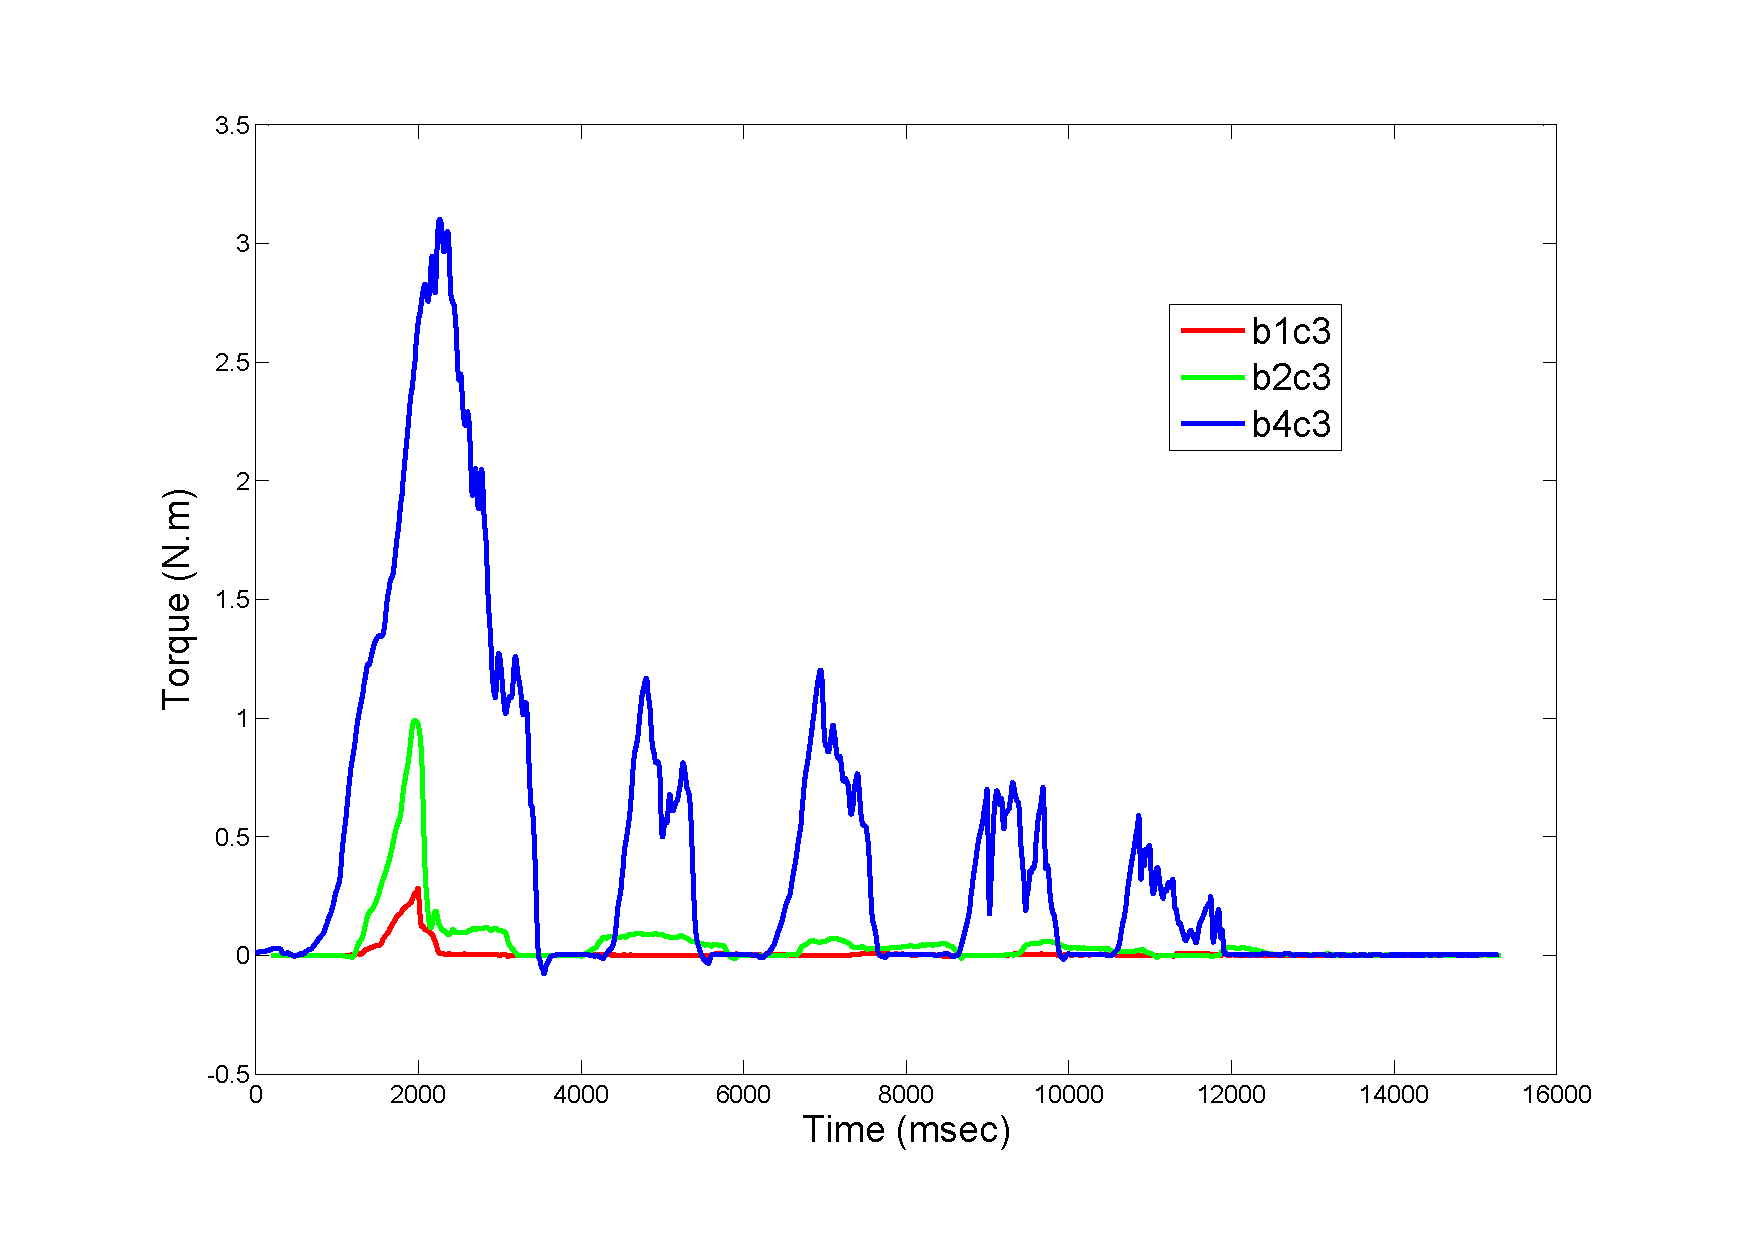
\includegraphics[width=8cm]{./fig/b1b3b4_time_T_2.pdf}#
  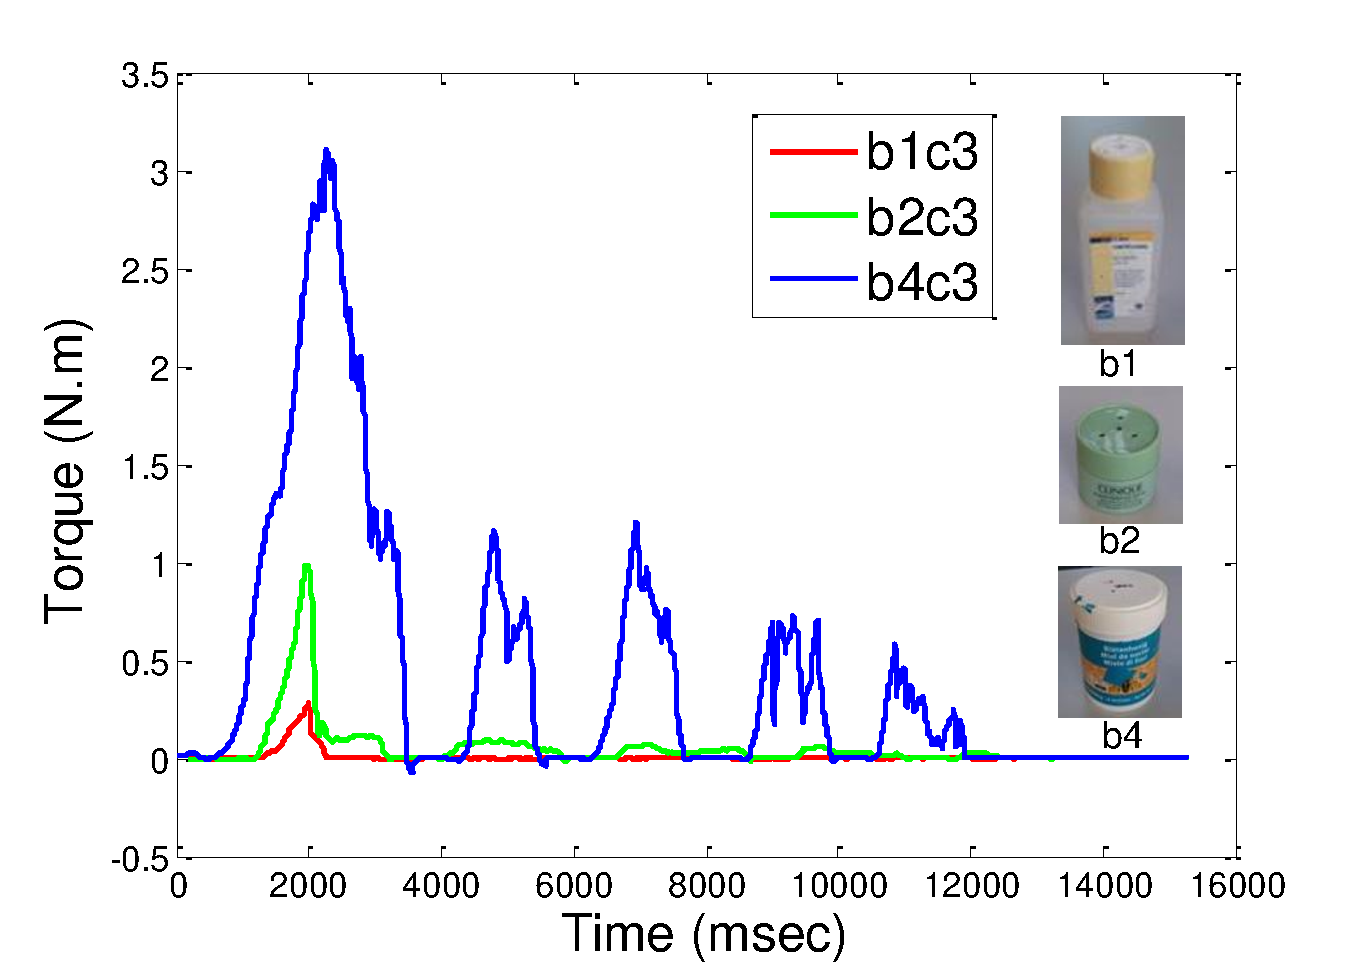
\includegraphics[width=8cm]{./fig/b1b2b4_time_T.pdf}
  \caption{ \scriptsize{Exert torque for opening three different bottles.}
}
\label{fig:bottlepatterns}
\end{figure}


\subsubsection{Demonstration in different task contexts}
\label{sec:exp_context}
The experiment starts with human demonstration. In order to explore different task contexts, we demonstrated the task with different setups, which are the combination of four different plastic bottles ($b1-b4$) and four different plastic caps ($c1-c4$) (Figure.~\ref{fig:b_c}).
According to the surfaces condition of the bottles and the caps, the difficulty of opening the bottles varies. $b1-b4$ are labeled by increasing difficulty. The bottle $b1$ is the easiest one, which originally contains body lotion. We lubricate bottle $b1$ with its body lotion to make it even easier. The bottle $b4$ is the most difficult one and it originally contains honey which is very sticky. We leave honey on the surfaces of $b4$ to make it more difficult. The difficulty is estimated qualitatively. It is judged according to the friction coefficient between the contact surfaces. Generally speaking, the friction coefficient between lubricated surfaces is smaller than between dry surfaces, while between smooth  surfaces is smaller than between sticky surfaces~\footnote{Precise value of friction coefficient between plastics varies by type of the plastic. According to an internet resource, the dry dynamic friction coefficient between plastic-plastic surface is 0.2-0.4 and the lubricated dynamic friction coefficient is 0.04-0.1 ( http://www.tribology-abc.com/abc/cof.htm)}. The $c1-c4$ are labeled by the increasing diameters of the caps.

%By the increasing order of the friction, the bottles are labeled as $b1$, $b2$, $b3$, $b4$ (in order to enlarge the variance of the friction coefficients, we put lubricant to the bottle $b1$ and rough the contact surface between the bottle and the cap of $b4$). By the increasing order of the diameters of the caps, they are labeled as $c1$, $c2$, $c3$ and $c4$.

We chose to vary the setups in surface condition and cap size as these are the main variances between different bottles effecting the control strategy. The intention is to see how does these two variables effect human behaviour. To this end, we ``combine'' the bottles and the caps by mounting the caps onto the ``actual caps'' of the bottles (Figure.~\ref{fig:setup}). To investigate the effects of different caps and different bottles separately, we conduct two groups of demonstrations: a fix bottle with 4 different caps ($b3c1, b3c2, b3c3, b3c4$) and a fix cap with 4 different bottles ($b1c3, b2c3, b3c3, b4c3$). Demonstrations on the first group allow us to explore human grasping strategies with different cap sizes. Demonstrations on the second group allow us to explore human control strategies in adapting to different bottle condition. In total, we have seven different setups for the human demonstration (Table~\ref{bottlesandcaps}).


\begin{figure}
  \centering
  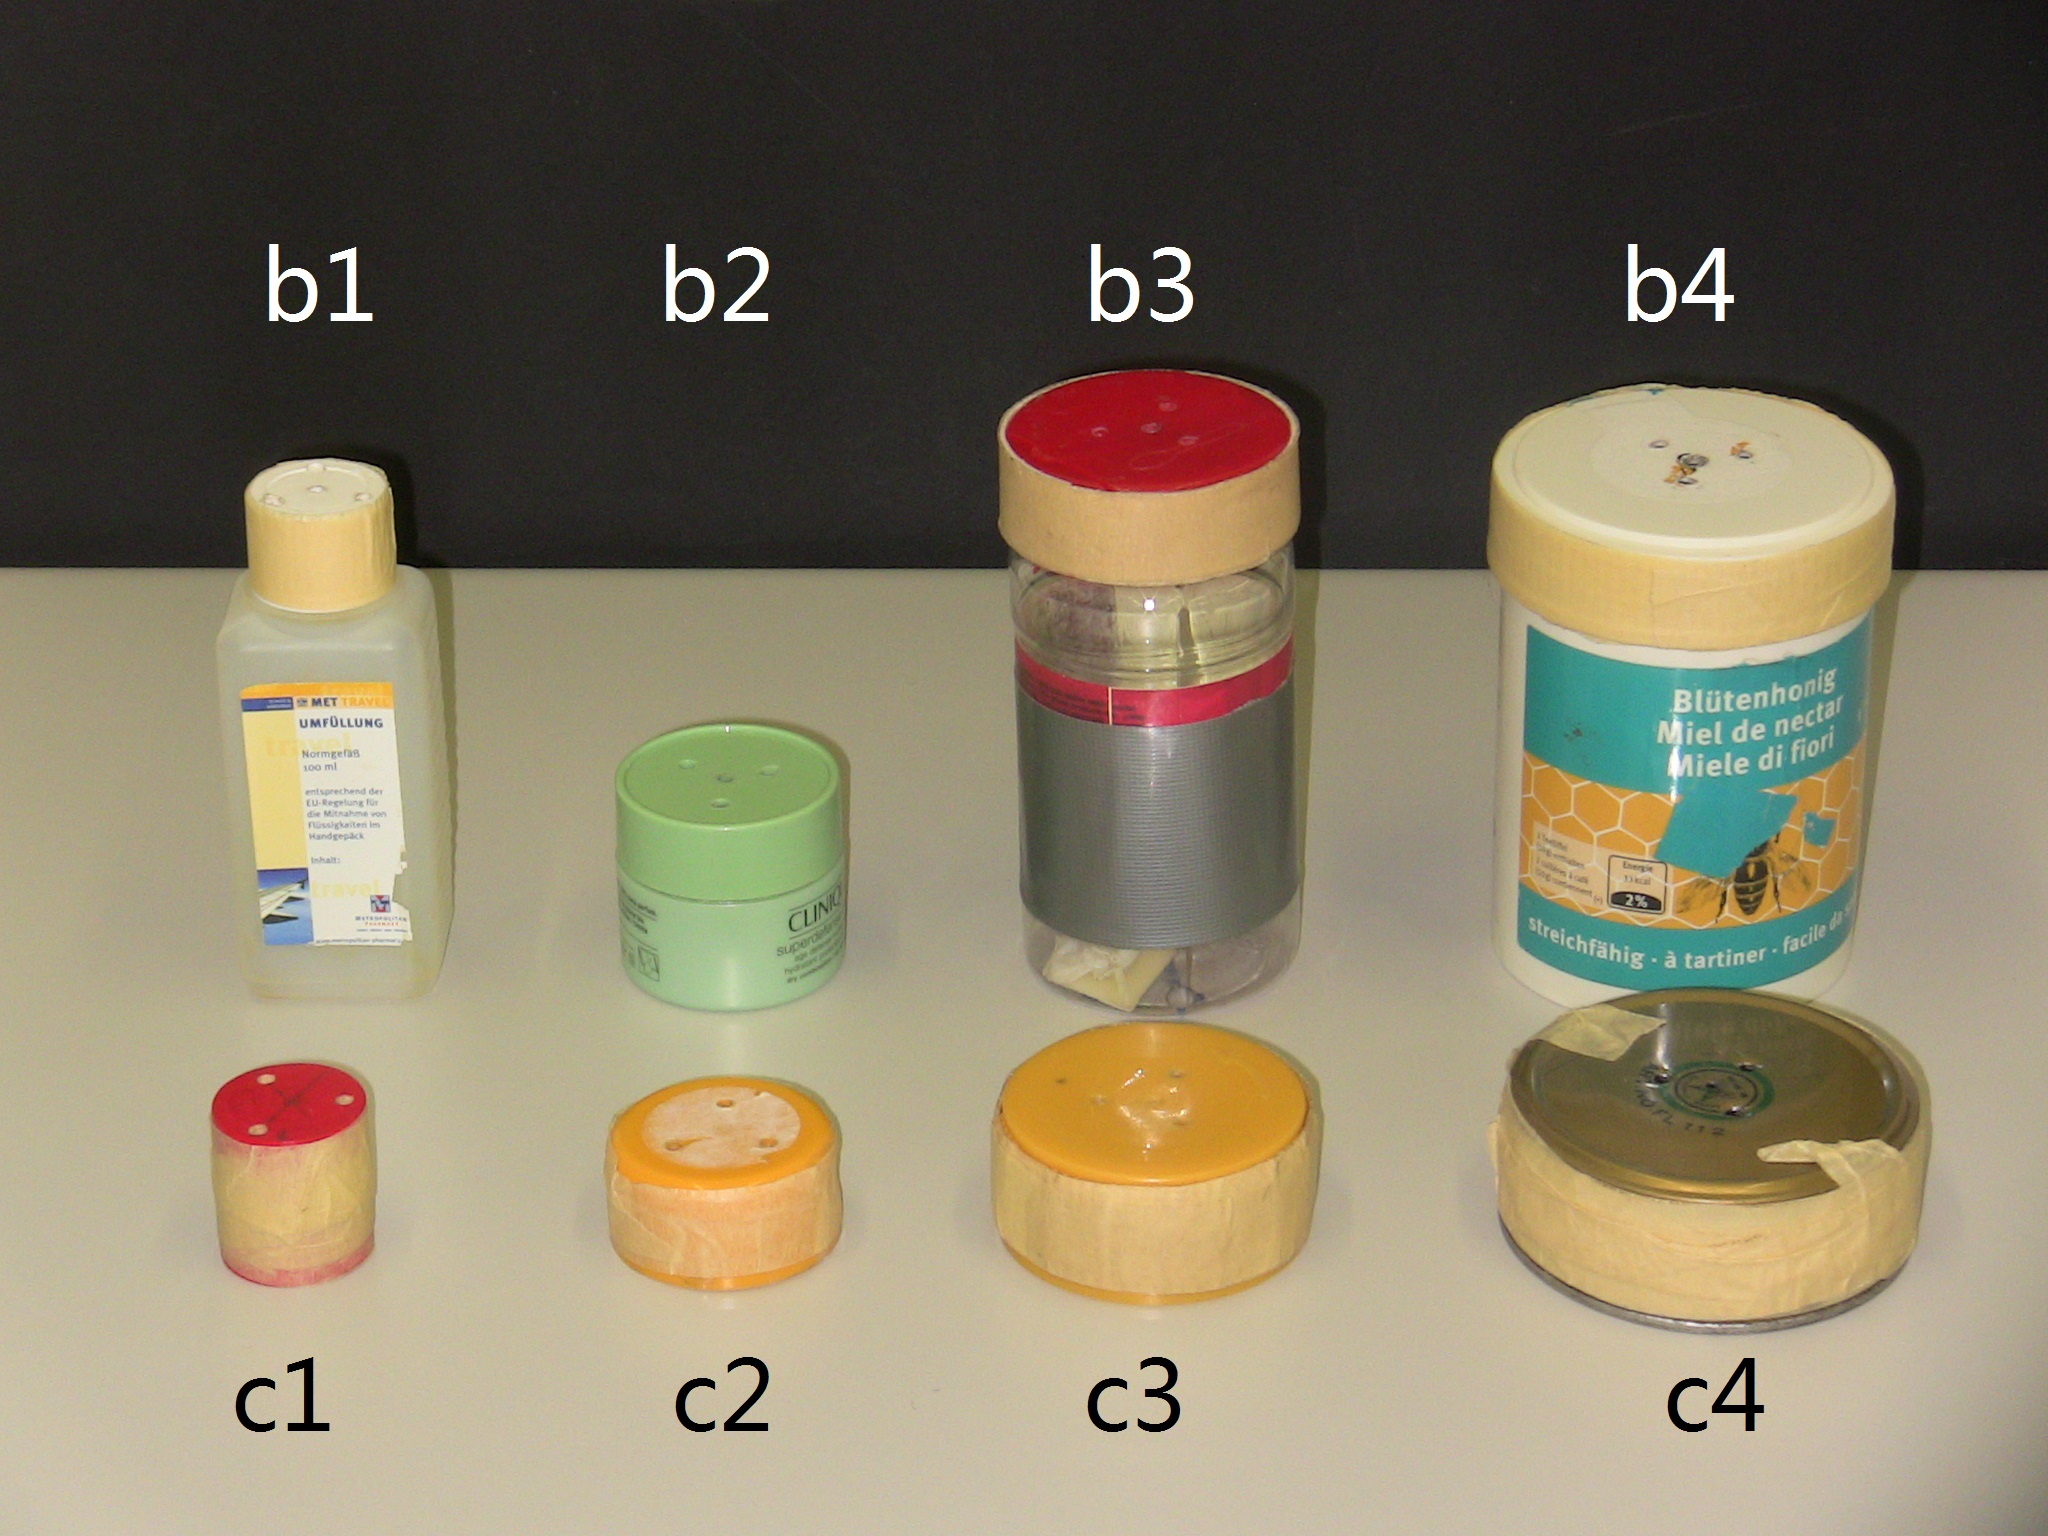
\includegraphics[width=5cm]{./fig/b_c.jpg}
  \caption{ \scriptsize{Bottles and caps for human demonstration. From left to right: b1 c1, b2 c2, b3 c3, b4  c4}
}
\label{fig:b_c}
\end{figure}



%\begin{figure}
%\centering
%    \subfloat[\scriptsize{}]  {\includegraphics[width=0.8in]{./fig/spr.jpg}}
%    \hspace{0.07in}
%    \subfloat[\scriptsize{}] {\includegraphics[width=0.8in]{./fig/box123.jpg}}
%%    \hspace{0.01in}
%\caption{\scriptsize{(a) A spray flask. (b) A spray flask approximated by 3 boxes.}}
%\label{fig:spr}
%\end{figure}


% 25,42,56,80,110, c1-c5, mm
\begin{table}
\center
\begin{tabular}{p{1.5cm}|p{1cm} |p{1cm} |p{1cm} |p{1cm}}

%\backslashbox{}{}
                                & \parbox[c]{1em}{ 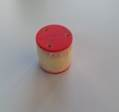
\includegraphics[width=1cm]{./fig/c1.jpg}}
                                & \parbox[c]{1em}{ 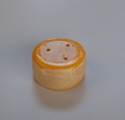
\includegraphics[width=1cm]{./fig/c2.jpg}}
                                & \parbox[c]{1em}{ 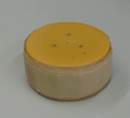
\includegraphics[width=1cm]{./fig/c3.jpg}}
                                & \parbox[c]{1em}{ 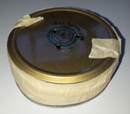
\includegraphics[width=1cm]{./fig/c4.jpg}}  \\
    & Cap 1 25$mm$ & Cap 2 42$mm$ & Cap 3 56$mm$ & Cap 4 80$mm$ \\
\hline
\parbox[c]{1em}{ 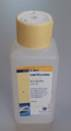
\includegraphics[width=1cm]{./fig/b1.jpg}} & & &b1c3 &\\
Bottle 1 & & & &\\
\hline
\parbox[c]{1em}{ 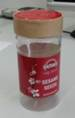
\includegraphics[width=1cm]{./fig/b2.jpg}} & & & &\\
%Bottle 2 & b2c1& b2c2& b2c3& b2c4\\
Bottle 2 & & & b2c3&\\
\hline
\parbox[c]{1em}{ 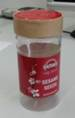
\includegraphics[width=1cm]{./fig/b3.jpg}} & & & &\\
%Bottle 3 & & & b3c3&\\
Bottle 3 & b3c1& b3c2& b3c3& b3c4\\
\hline
\parbox[c]{1em}{ 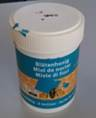
\includegraphics[width=1cm]{./fig/b4.jpg}} & & & &\\
Bottle 4 & & & b4c3&\\
\hline
\end{tabular}
\caption{Different setups of bottles and caps for demonstration. Bottle 1 to 4 are in increasing order of the difficulty to open. Cap 1 to 4 is in increasing order of the cap sizes, whose diameters are shown.}
\label{bottlesandcaps}
\end{table}

\begin{figure}
  \centering
  \subfloat[\scriptsize{}]  {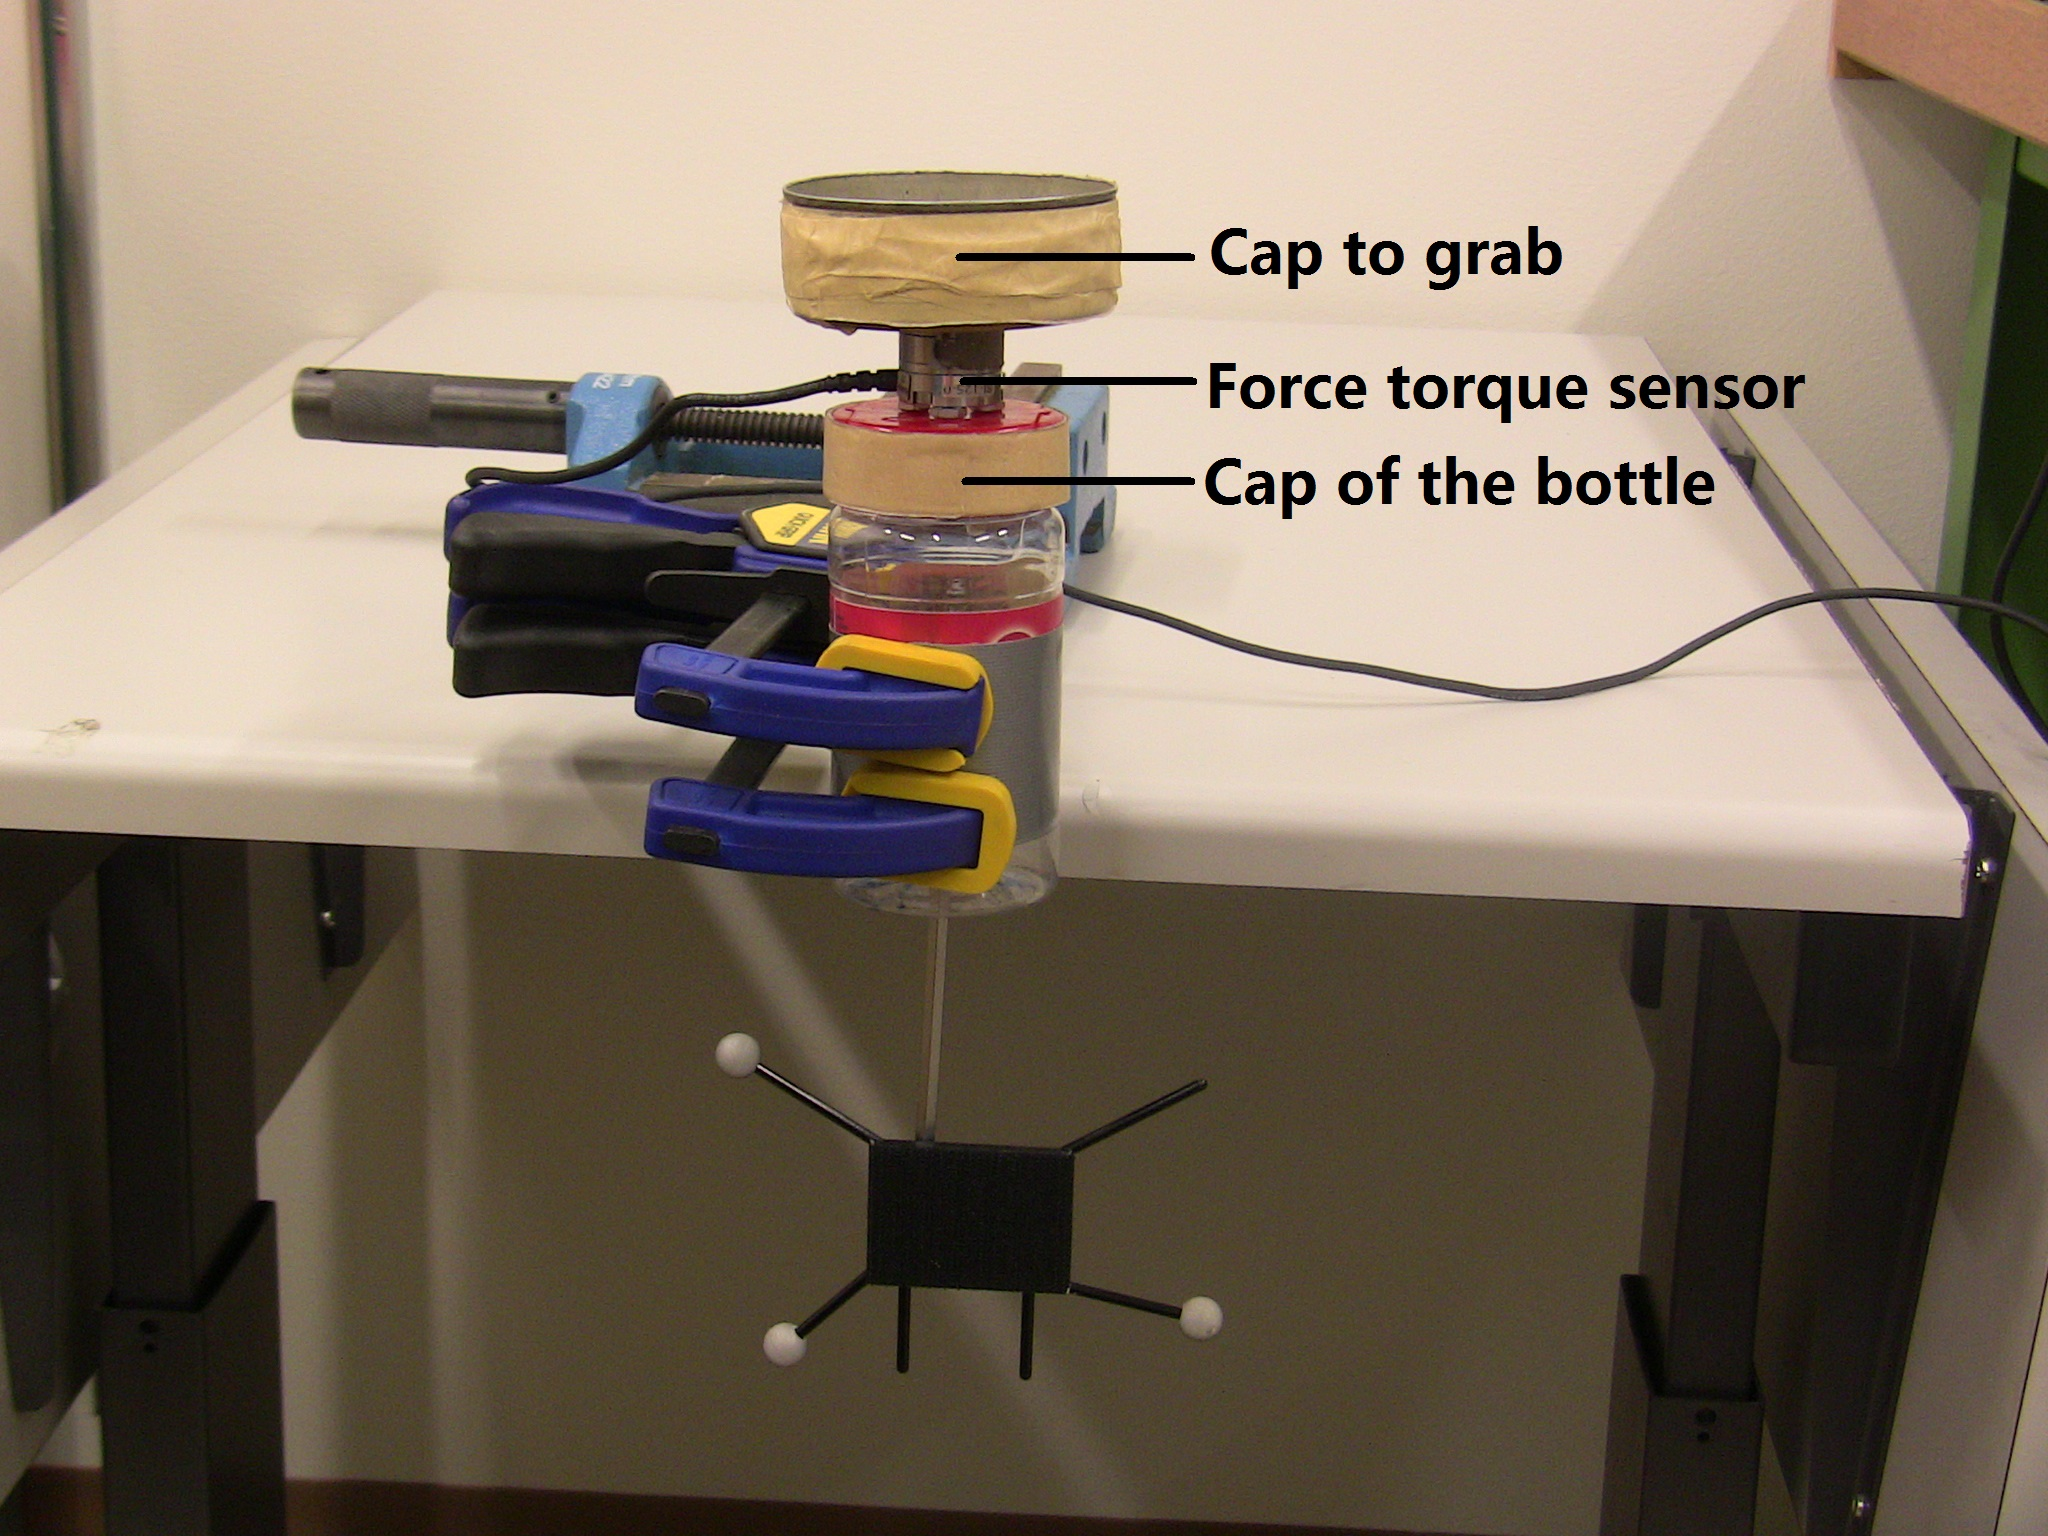
\includegraphics[width=5cm]{./fig/setup2_2.jpg}}
  \hspace{1cm}
  \subfloat[\scriptsize{}]  {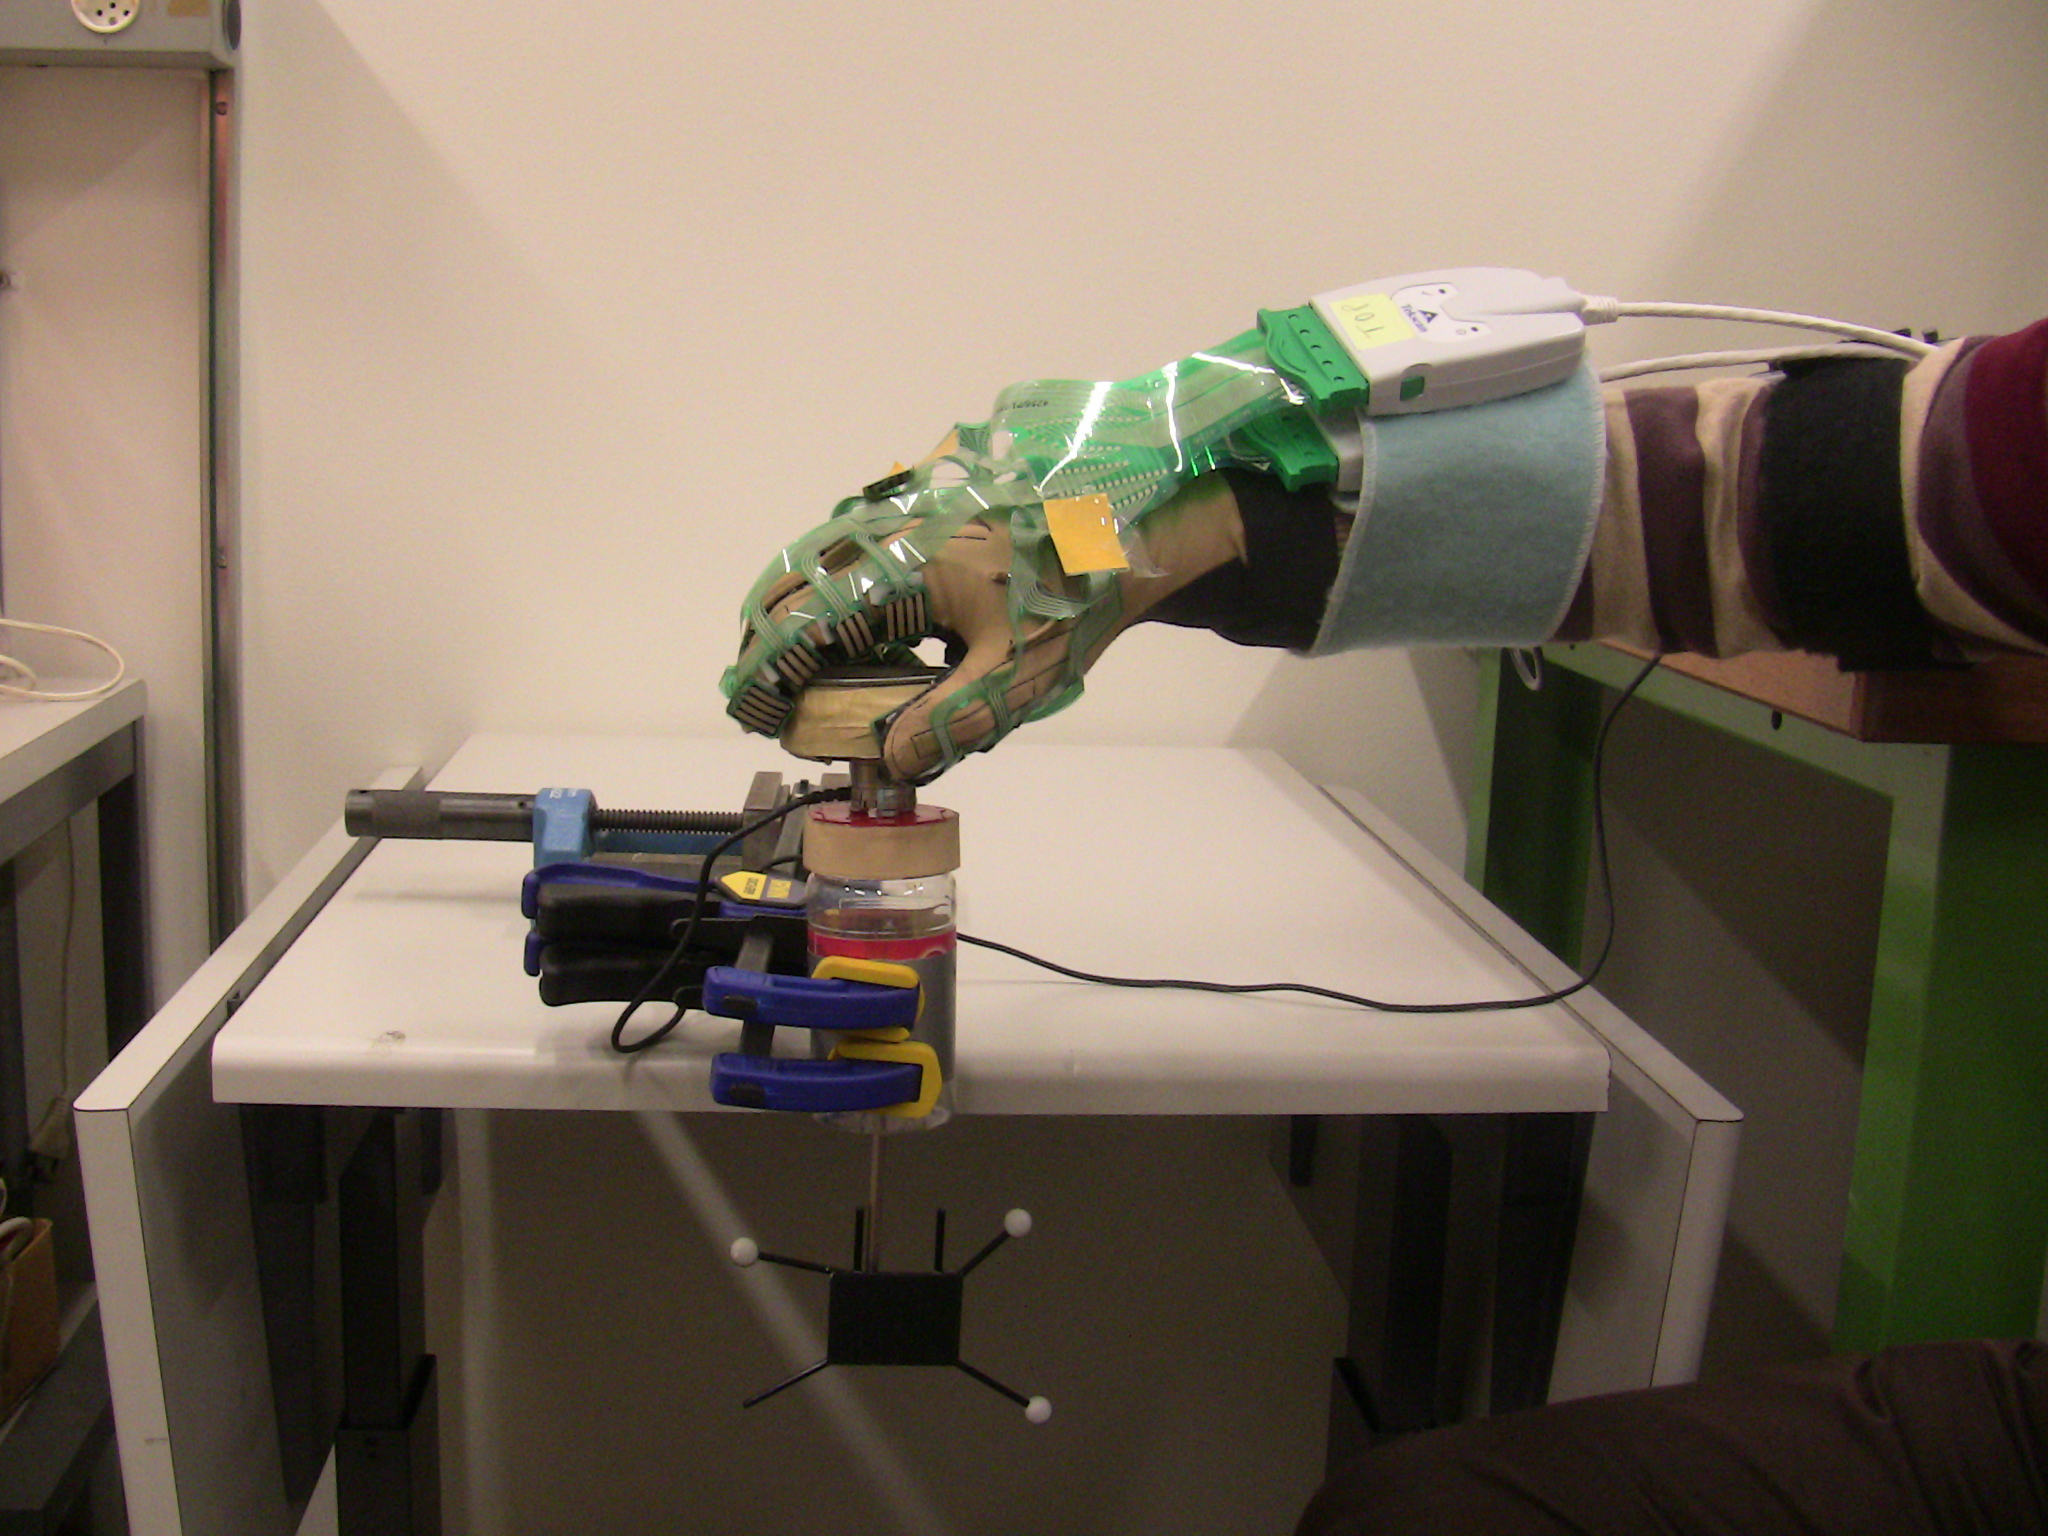
\includegraphics[width=5cm]{./fig/demo.jpg}}
  \caption{ \scriptsize{Experimental setup for the task of opening a bottle cap. (a) Setup b3c4: bottle 3 combined with cap 4 (cap to grab). A force-torque sensor is mounted between the ``cap of the bottle'' and the ``cap to grab'', so that the exert force and torque can be measured. A set of Optitrack markers are connected with the cap to record the displacement of it. The bottle is fixed on a table. (b) Human demonstrating opening a bottle cap. To avoid extra torque, only one hand is used during the demonstration. Human grip the cap from the top and apply torque to the system. }
}
\label{fig:setup}
\end{figure}

\subsubsection{Sensors}
\label{sec:sensor}
In each setup the demonstrator demonstrates the task of opening bottle cap three times. Before each demonstration, the bottle is tighten with the cap with the same scale of tightness. In total we recorded 21 sets of demonstrations. In this section, we explain how did we record these demonstrations by sensors.



As explained in section~\ref{sec:objectlevel}, we focus on the tuple $\{\tau,F,s\}$ of the task. Three different set of sensors are used in the experiment to capture them:

\begin{enumerate}
\item Force torque sensor\footnote{https://www.ati-ia.com/} for exert torque ($\tau$);
\item OptiTrack\footnote{http://www.naturalpoint.com/optitrack/} for cap displacement ($s$);
\item Tekscan\footnote{http://www.tekscan.com/} for exert force ($F$).
\end{enumerate}

Data from these three sensors stream from three different channels. Due to the hardware limitation the raw data steam from different channels do not come at the same time, and are not recorded in a regular frequency. To synchronize the data, we produce a synchronization signal at the beginning of each demonstration: the demonstrator tap on the cap three times. The movement of the hand and impulses on the cap produce simultaneous pulses in all three channels. After recording, the data from different channels are synchronize by aligning the synchronization signal.

In this task, the turning torque is the essential variable. This is measured and recorded by a ATI force torque sensor. It is mounted between the bottle and the cap (Figure.~\ref{fig:setup}). During the task, the demonstrator grab the cap on the top of the force-torque sensor and apply torque to open the bottle mounted below the sensor. As the bottle is fixed on the table, the movement of the cap is restricted on the rotation along the bottle's axis. Under the approximation of zero angular momentum, the reading of the sensor shows the force and torque applied on the cap. Besides the torque, force applied to the z-axis direction is also recorded for the purpose of synchronization (Section~\ref{dataanalysis}).

We track the displacement of the cap by a motion tracking system OptiTrack. The OptiTrack system track movement by the infrared reflecting markers attached on the object. In order to avoid obstacle of the demonstration, we attach markers to a stick, which is fixed to the cap from one end and the other end coming out from the bottom of the bottle (Figure.~\ref{fig:setup}). We also recorded the human hand movement, by tracking the markers attached to the human hand. The movement of human hand is used later for synchronization (Section~\ref{dataanalysis}).

During the task, human also apply grip force on the cap in order to grasp it firmly for turning. This force can not be sensed by the force torque sensor. Therefore, we used a pressure sensor (Tekscan Grip System) for measuring the human grip force. The Tekscan Grip System is a flexible tactile pressure sensor that can be built into a glove. It has 18 patches of sensors to covert the human hand front surface. For manipulation human use not only the front surface, but also the side surface of our fingers. In order to measure the force applied by those surfaces, we mount two sets of Tekscan Grip System sensors onto a glove to cover also the side surfaces (Figure.~\ref{ftsensor}). The method of mounting the sensors to the glove is detailed in~\citep{deSouza2014}. With different sizes of the caps or in different stages of the task, the way human grasp the cap varies, e.g. using 2 fingers to grip the smallest cap c1 and using 4 fingers to grab the biggest cap c4. The used patches in each grasps are recorded. In the computation of the total grip force, only the used patches are taken into account. All patches are calibrated to read in the unit of $N{\cdot}m$.


\subsection{Data Analysis}
\label{dataanalysis}
% Data: how to compute the cap displacement. Hand position. compute contact force. Figure of tekscan!!
In this section we explain how we manage the raw data and extra training data.
The raw data from the three sensors stream in three separated channels. They have different formats and hence are handled differently.

\paragraph{\textbf{Exert torque}}
\label{ftsensor}
As the movement of the cap is restricted to the rotation along the z-axis, we concern only the torque applied in this direction.  %(Figure.~\ref{fig:ftsensor}).
Other concerned dimension is the force applied in the z direction. The three taps on the cap before each demonstration will create three pulses in the z direction and hence is used for synchronization.


\paragraph{\textbf{Object displacement}}
\label{sec:optiktrack}
%With 3 markers attached with the object, OptiTrack is able to track both the object's translation and rotation. This is
From the OptiTrack, the cap's displacement is originally expressed in the position vector and the rotation matrix. To compute the angular displacement of the cap by the ration matrix of the cap, and compute the hand movement by the position vector of the hand. The accumulated angular displacement is used to learn the model and the hand movement is used to synchronize the data. % (Figure.~\ref{fig:optitrack}).
%
%\begin{figure}
%  \centering
%  %\subfloat[\scriptsize{}]  {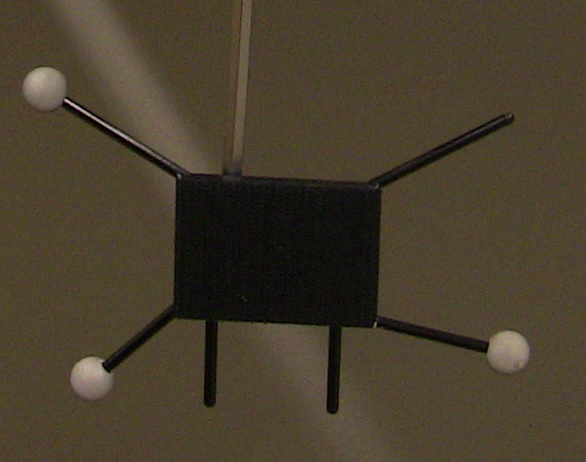
\includegraphics[width=4cm]{./fig/marker.jpg}}
%  %\hspace{0.5cm}
%  %\subfloat[\scriptsize{}]  {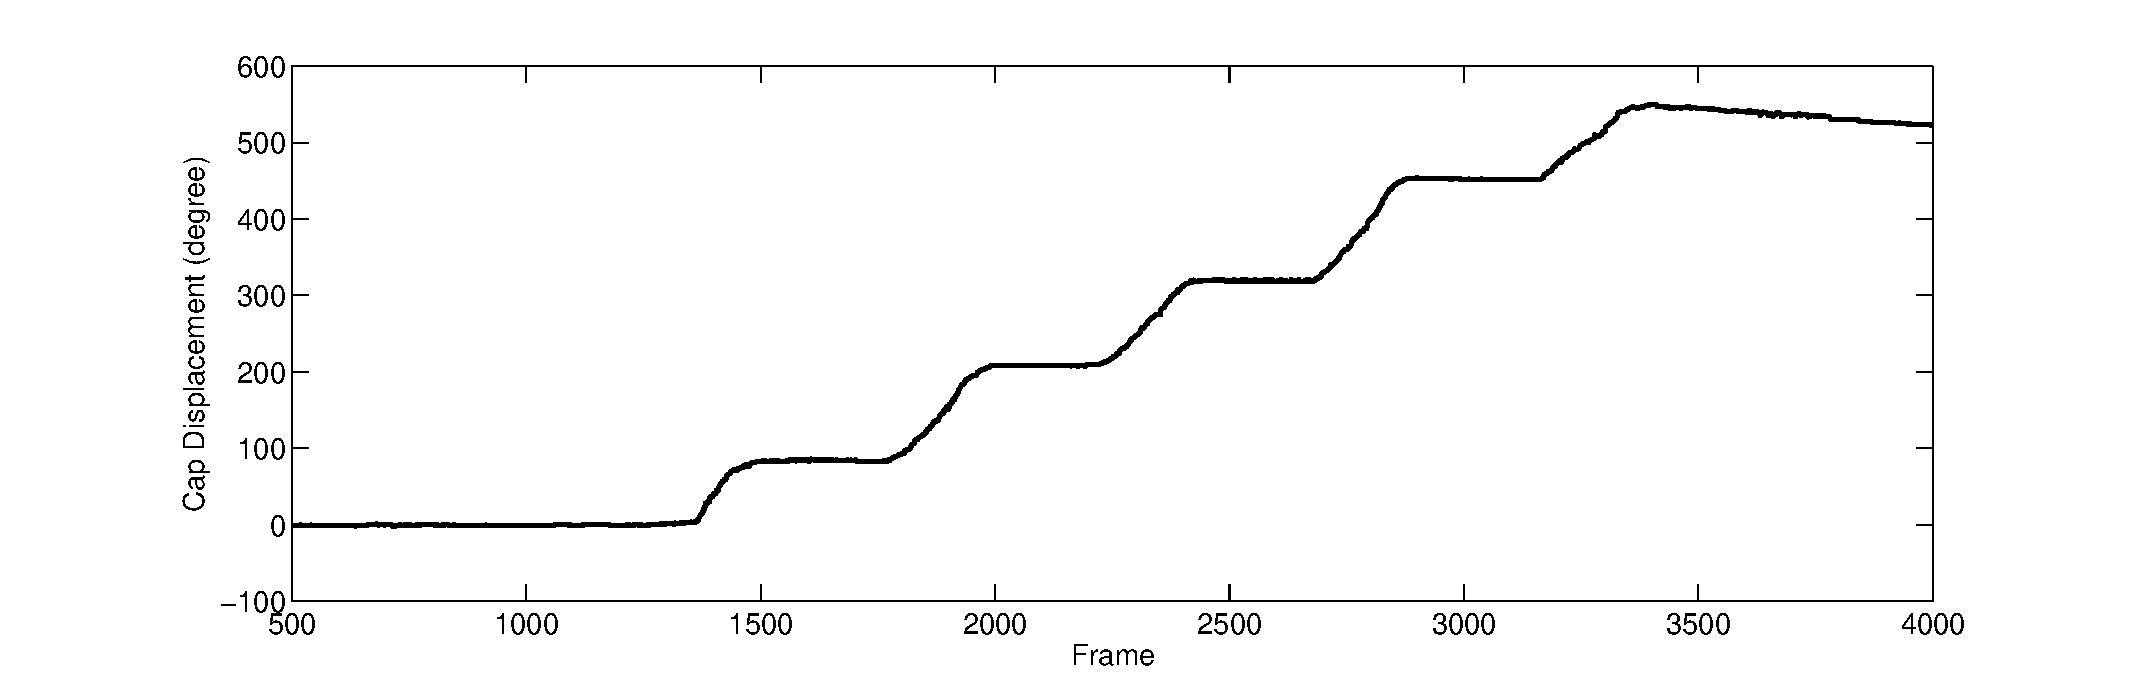
\includegraphics[width=13cm]{./fig/b3c2_5_s.eps}}
%  %\caption{ \scriptsize{Tracking cap displacement. (a) OptiTrack markers. (b) }}
%  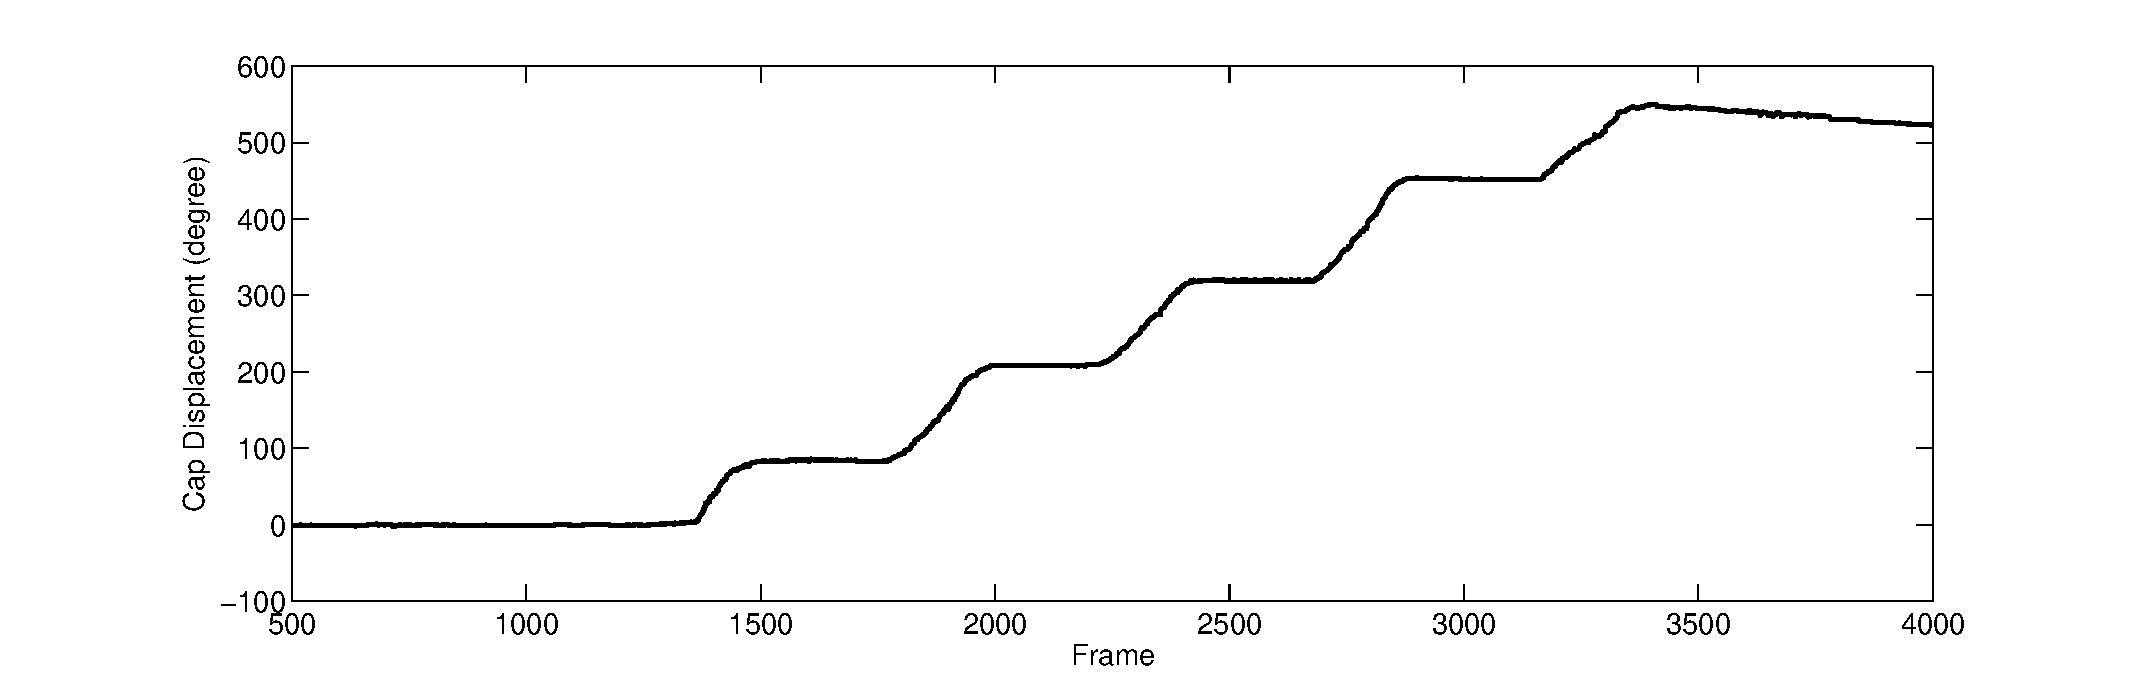
\includegraphics[width=8cm]{./fig/b3c2_5_s.eps}
%  \caption{\scriptsize{Cap angular displacement during one demonstration (of b3c2). }}
%\label{fig:optitrack}
%\end{figure}



%\begin{figure}
%  \centering
%  %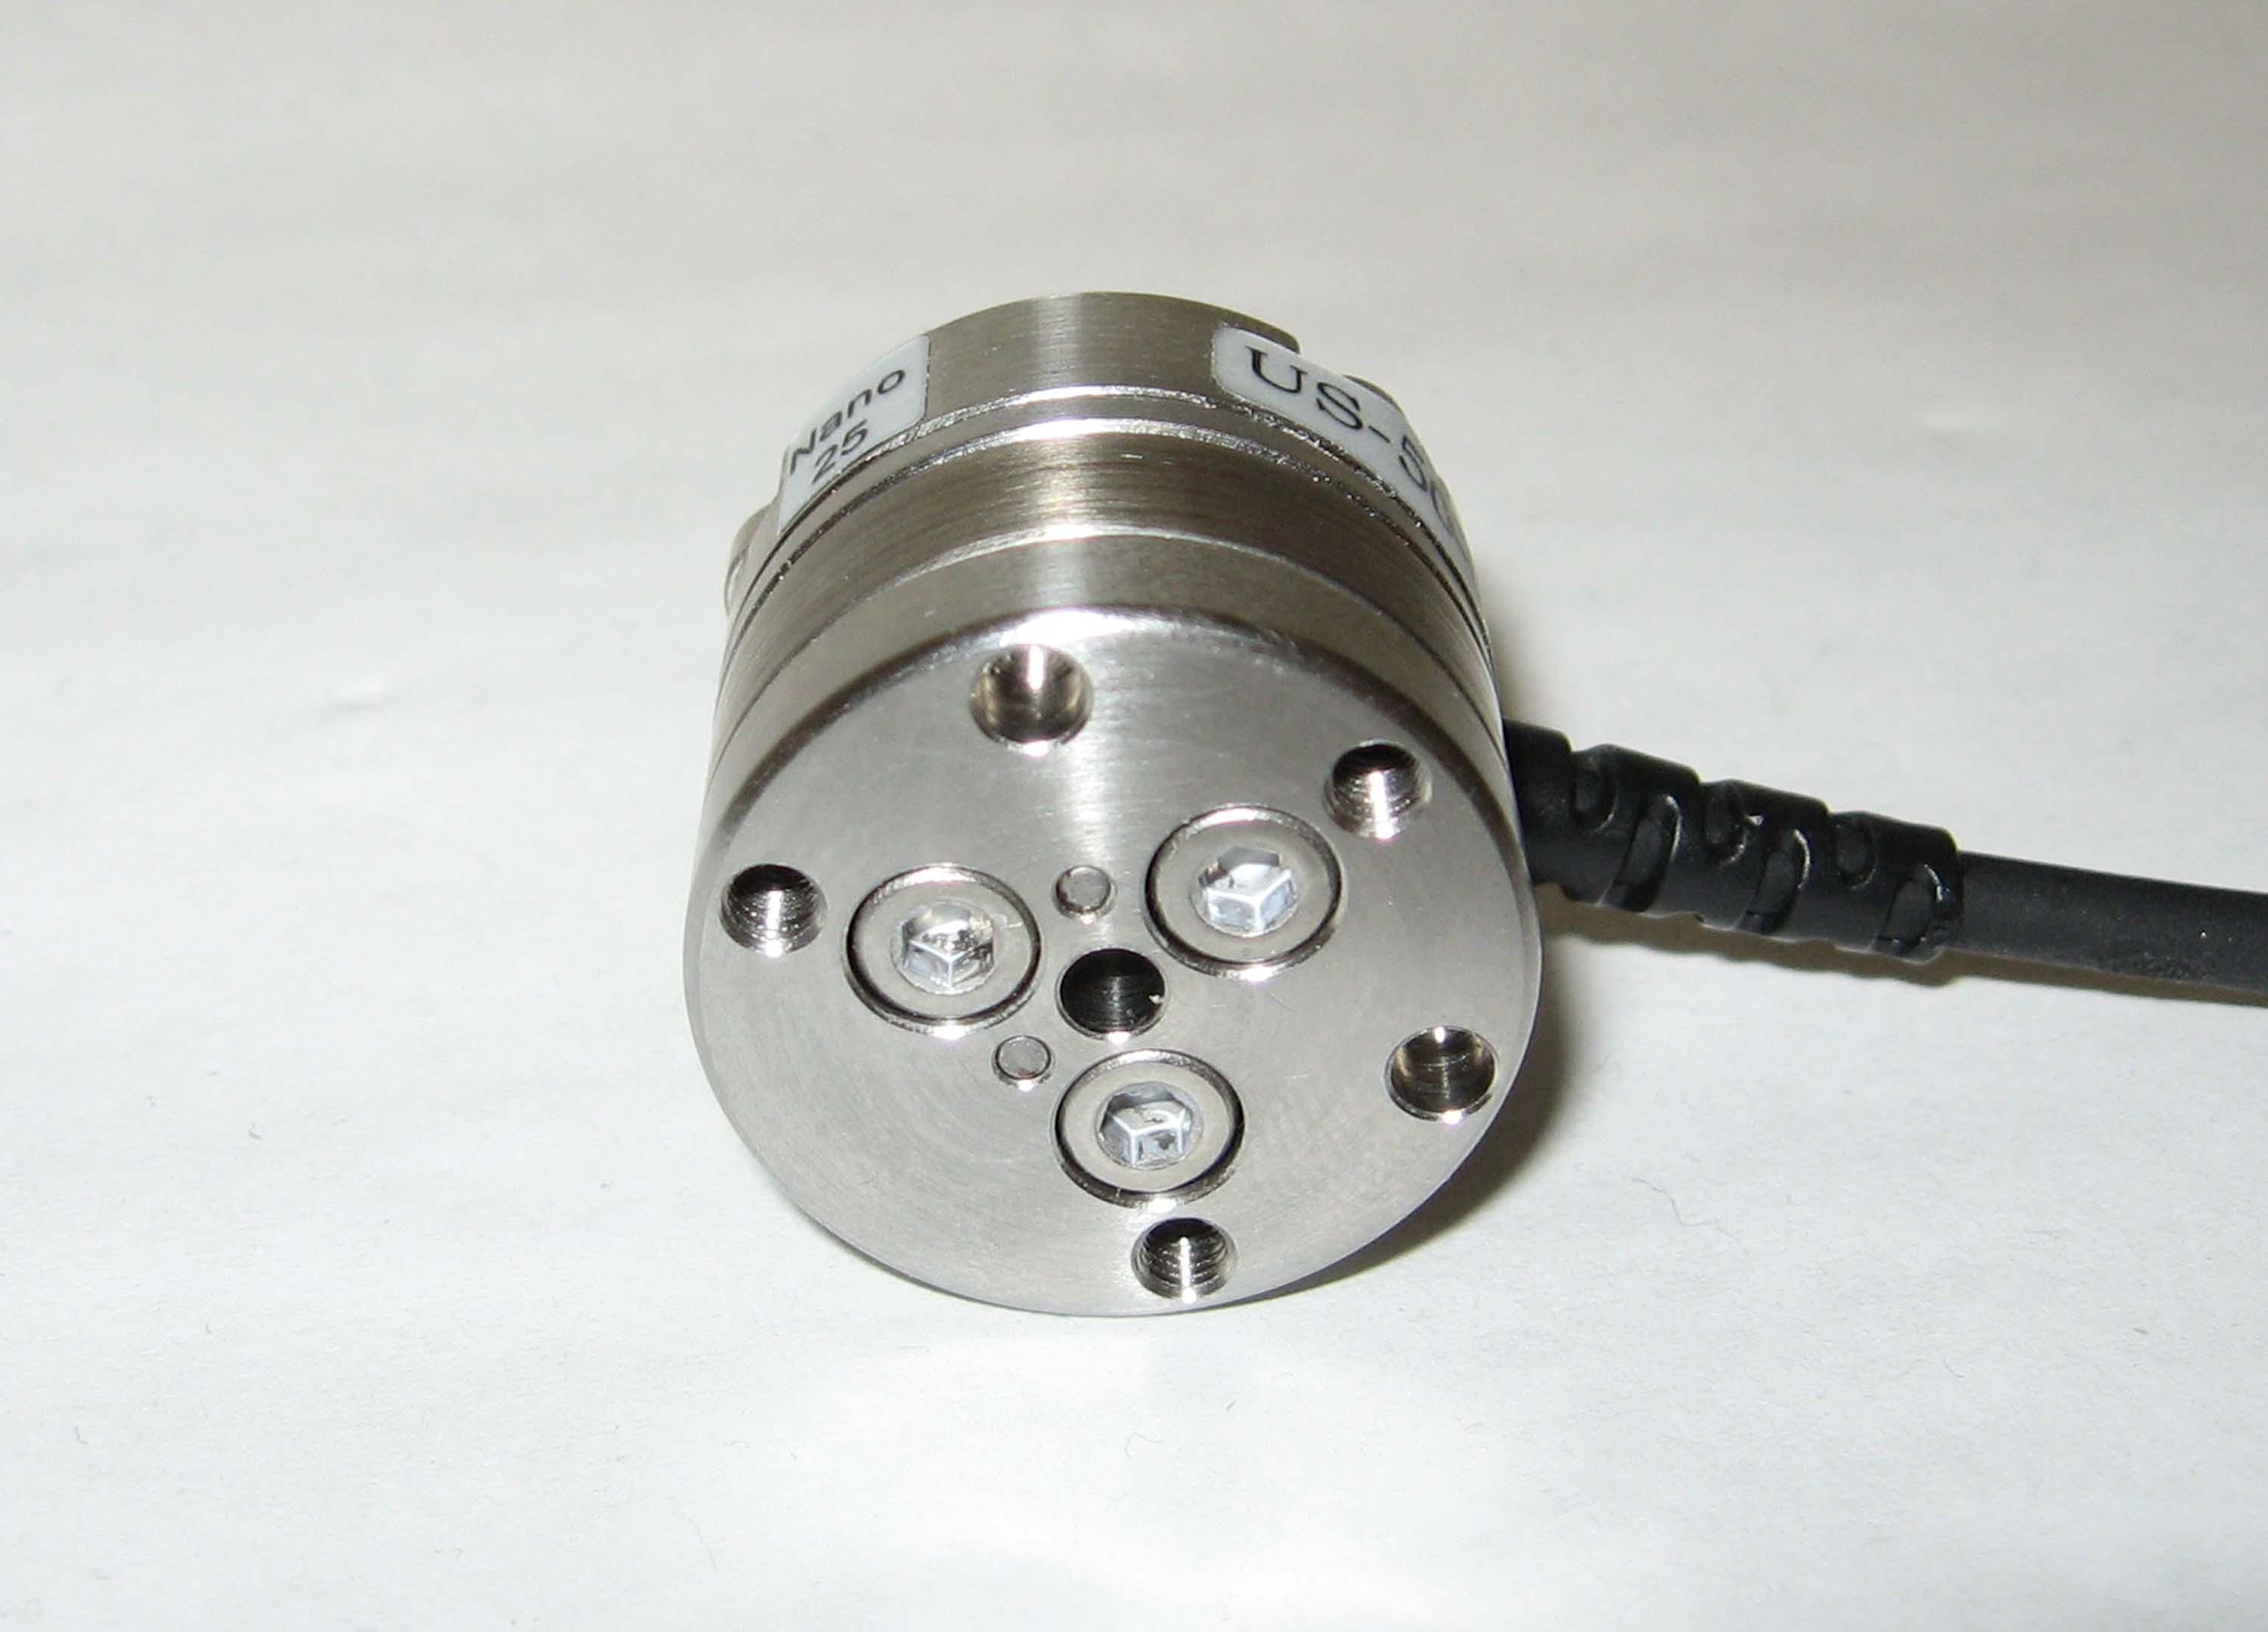
\includegraphics[width=4cm]{./fig/Nano25-E.jpg}
%  %\vspace{0.2cm}
%  %\subfloat[\scriptsize{}]  {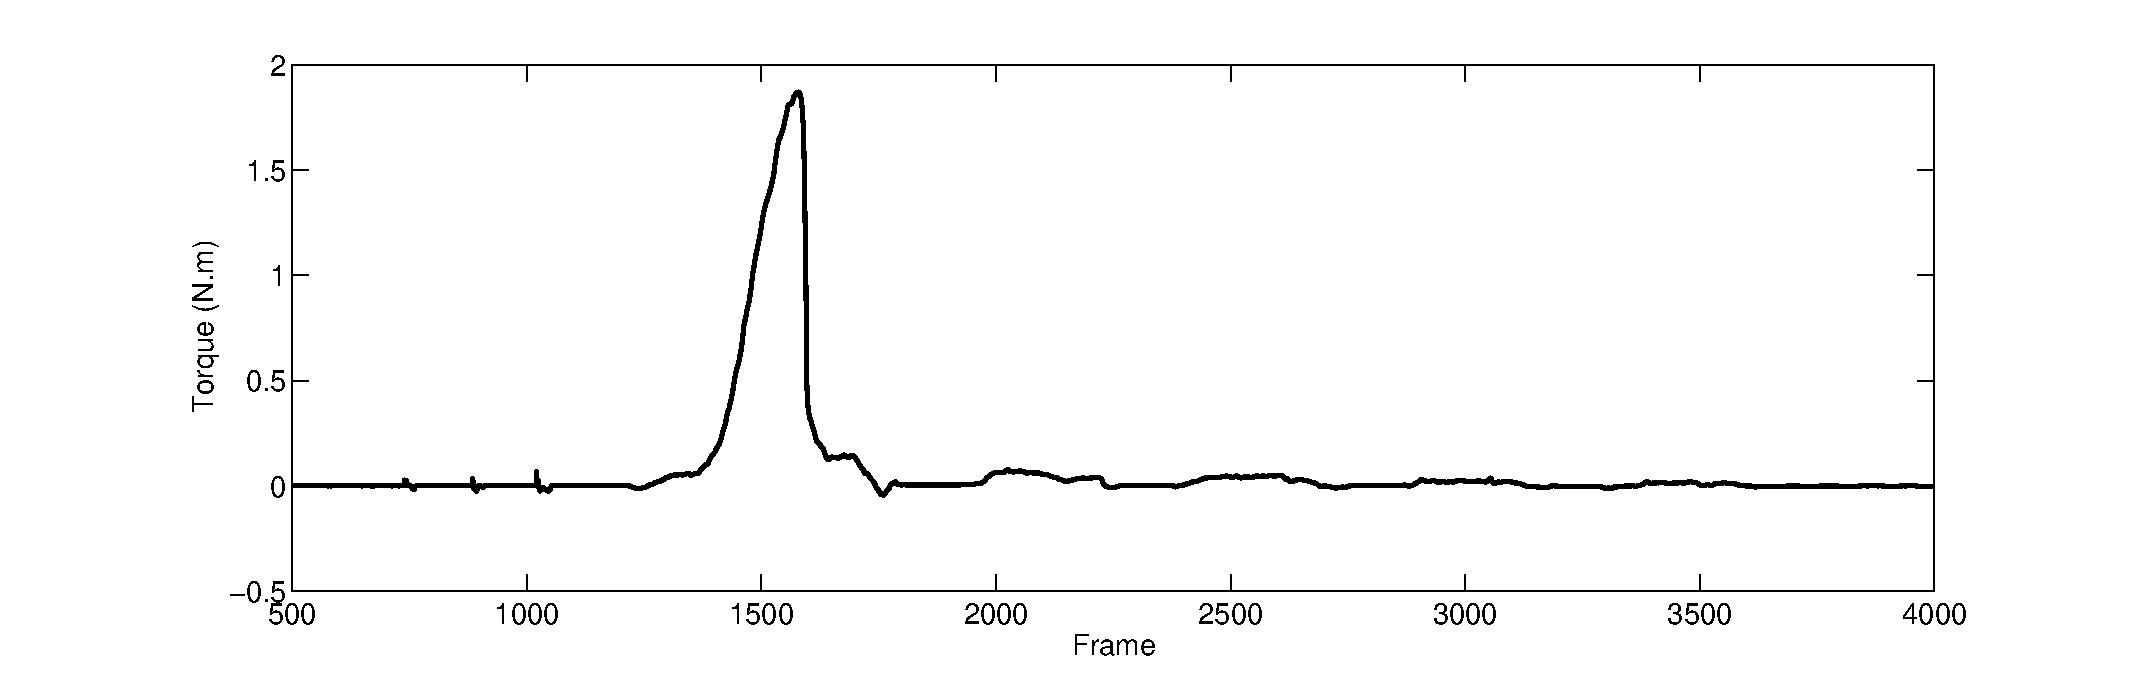
\includegraphics[width=13cm]{./fig/b3c2_5_T.eps}}
%  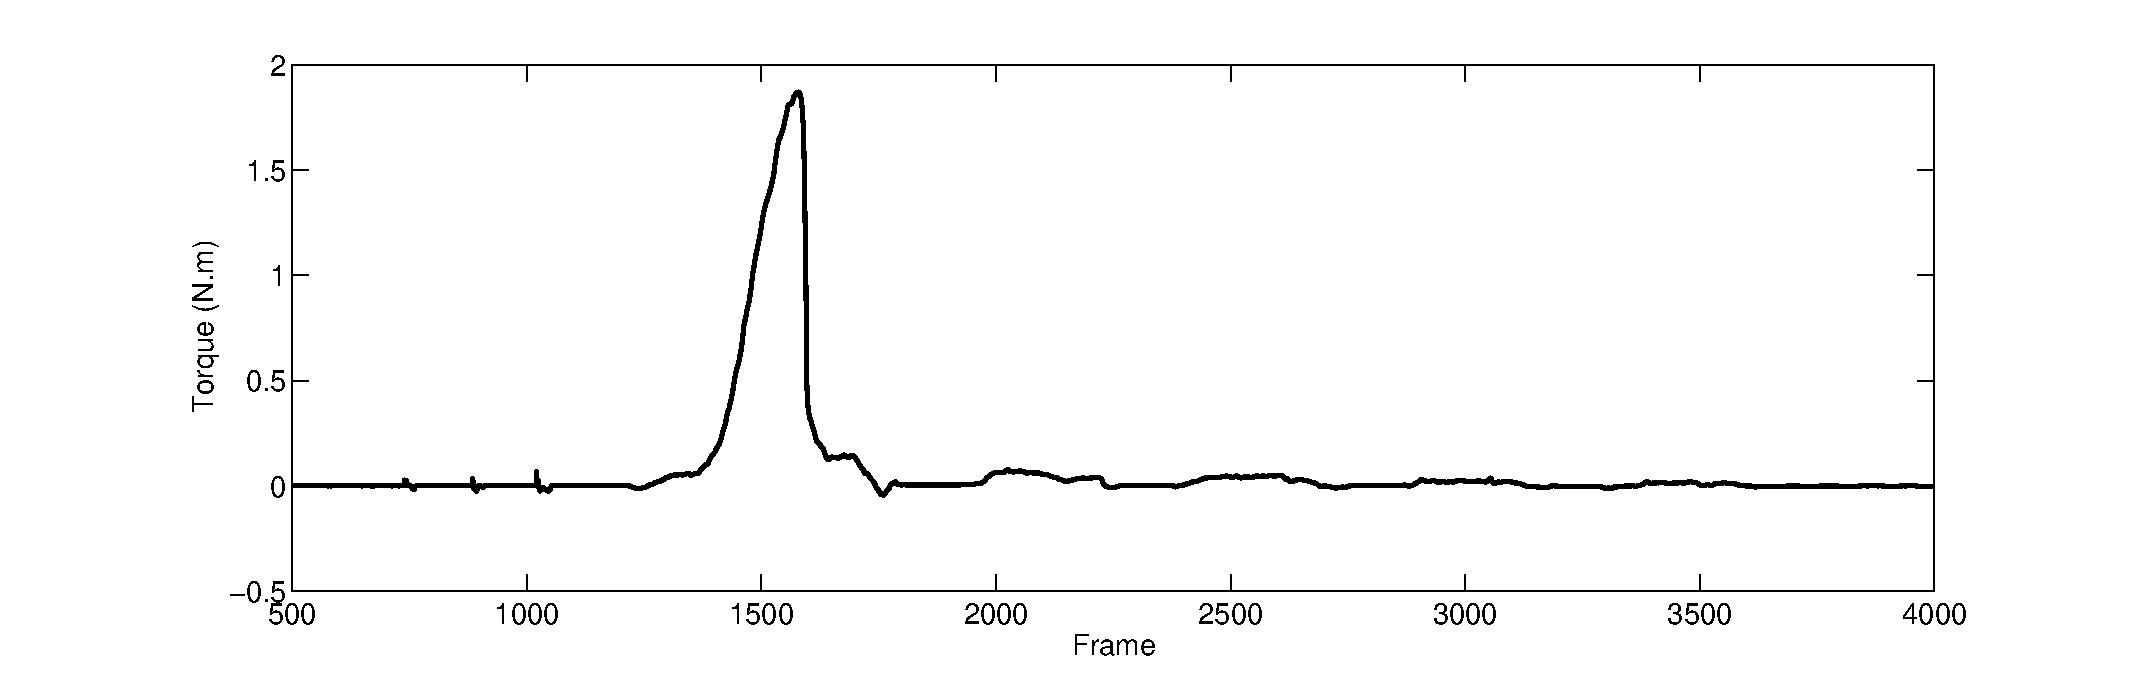
\includegraphics[width=8cm]{./fig/b3c2_5_T.eps}
%  %\caption{ \scriptsize{Force torque sensor. (a) Nano25-E force torque sensor. (b) Exert torque during one demonstration (of b3c2). }}
%  \caption{ \scriptsize{Exert torque during one demonstration (of b3c2). }}
%\label{fig:ftsensor}
%\end{figure}

\paragraph{\textbf{Grip Force}}
\label{tekscan}
As mentioned in previous section, we use two set of Tekscan to cover the front and the size of the human hand. This enable the demonstrator to use any grasp they like for the task, not restricted to using the first three fingers as most of the other grasp experiment. In each type of grasp, the reading from the patches contacting with the cap are summed and multiplied by their surface area to compute the total grip force.% (Figure.~\ref{fig:ftsensor}).

%\begin{figure}
%  \centering
%  %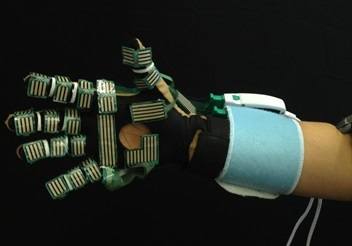
\includegraphics[width=5cm]{./fig/texscan2.jpg}
%  %\hspace{0.2cm}
%  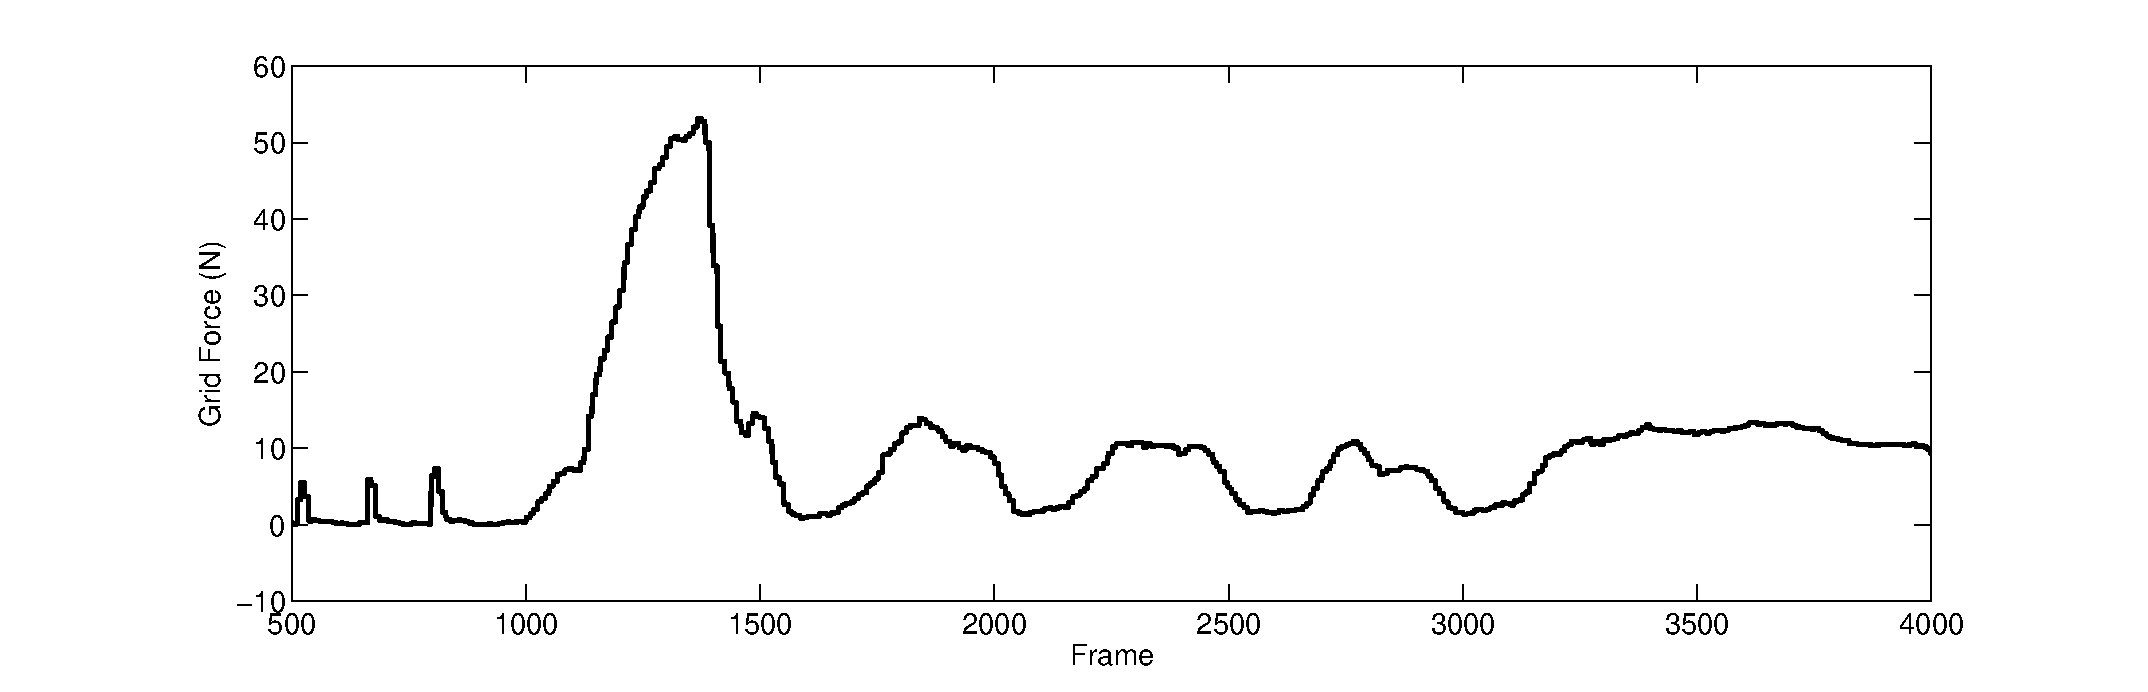
\includegraphics[width=8cm]{./fig/b3c2_5_F.eps}
%  %\caption{ \scriptsize{Tracking cap displacement. (a) Tekscan mounted on a glove. (b) Total grib force applied by different parts of the fingers in on demonstration. }}
%  \caption{ \scriptsize{Total grib force applied by different parts of the fingers in one demonstration  (of b3c2). }}
%\label{fig:ftsensor}
%\end{figure}

Data from these three channels is synchronized by aligning the synchronization pulses. The time of the last detected pulse is set to the zero reference point. After synchronization we re-sample all the temporal sequences to 100Hz. Hence each single data point is synchronized. Finally, we filtered the noise by a low pass filter. Figure.~\ref{fig:3channels} shows an example of the data from three different channels.




\begin{figure}
  \centering
  \hspace{-0.5cm}
  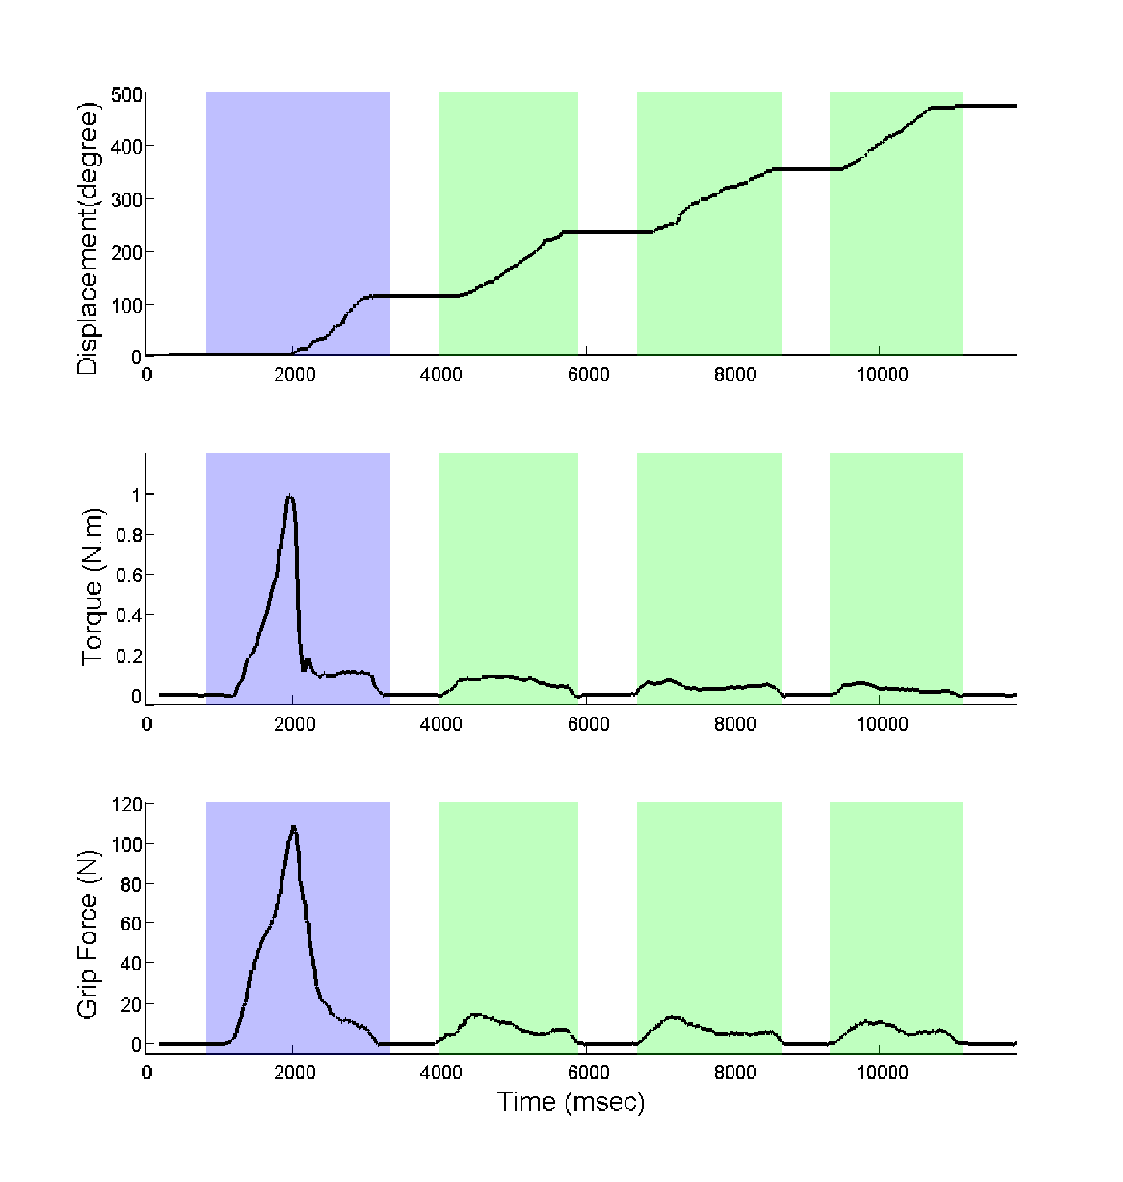
\includegraphics[width=9cm]{./fig/b3c2_1_sTF.pdf}
  \vspace{-0.5cm}
  \caption{ \scriptsize{Aligned data of all three channels. Highlighted parts mark the turning process: blue blocks denote the first cycle, i.e. the phase I, and green blocks denote the later cycles, i.e the phase II. Phase I is significantly different from the phase II.}
}
\label{fig:3channels}
\end{figure}

% Only turning cycle
In this task we focus on the turning stage of each cycle. More specifically, we focus on the data starts from the moment that the fingers contact the cap and end at the moment that the turning is finished and the cap is released. The reaching and releasing cycles do not involve contact with the environment and hence are not concerned here.
% segmentation is not our job
In order to collect data from only the turning cycles, we trim the data by the contact single: only the sequence with non-zero contact force will be kept.\footnote{In this task the segmentation is done manually. The data can also be segmented by other algorithms but here we do not focus on task segmentation.} The trimmed sequences are labeled by their setups and the order of their appearance, e.g. the 1st cycle of the bottle 1 with cap 3 is labeled by $b1c3\_1$.

As can be seem from Figure.~\ref{fig:3channels}, there are dramatic difference between the cycle one and the rest of the cycles: the exert force and torque are much higher in the first cycle than in the other cycles. This is caused by the difference between the static friction and the kinetic friction. At the beginning of the task we have to first break the contact between the bottle and the cap. The friction we need to break at this stage is decide by the static FCO. Once the cap starts to move, the FCO between bottle and cap transits to kinetic FCO, which is usually smaller than the static FCO for the same surface condition. As a result, the torque and hence the grip force required to turn the cap decrease in the later cycles. This phenomenon implies that at lease two modules are needed for this task. In the later section we will discuss these two phases separately and refer the cycle one as ``phase I'' and the later cycles as ``phase II''.

In different demonstrations, the number of cycles used to open the cap is different, varying from four to six. The pattern of the later cycles  are similar as the demonstrator just repeat the same strategy to rotate the cap. For training, we take the first four cycles from each of the demonstration. This results in 84 time series in total for the learning.

%% what was recorded
%In each demonstration, data from first time the hand grab the cap to the cap is finally open and lifted, was record. Opening bottle cap is a cyclic task, each cycle of which includes reaching, turning and releasing stages. Depending on the tightness of the cap, a few cycles need to be done before the bottle is open. In this task we focus on the turning stage of each cycle, which start from the time that the fingers contact the cap and end at the moment that the turning is finished and the cap is released. During the turning cycles, force and torque are applied to the cap in order to break it's contact with the the bottle and the dynamics of the system changes diametrically. Our goal is to learn a model to encode human's strategy to cope with the abruptly changing environment during the turning cycle. The reaching and releasing cycles do not involve contact with the environment and hence we omit them.







\subsection{Learning Modules}
\label{learning}
%\begin{itemize}
%  \item First hierarchical clustering \ldots
%  \item Find out number of models \ldots
%  \item Second build GMM for each of the model \ldots
%\end{itemize}

In this section, we explain how do we encode the training data into a few different modules. As mentioned in Section~\ref{sec:learn}, the first step is to cluster the data and find out the number of modules required in this task.

\subsubsection{Data clustering}
To cluster the 84 time series $Q\{s,\tau,F\}$ obtained from human demonstration, we first computed the distance between each pair of them by the DTW technique. As this task is time independent, ``warping'' of the data in the dimension of time does not effect the control policy encoded in the time series. The distances between each pair of the time series is shown in the heatmap (Figure.~\ref{fig:heatmap}). As can be told from the heatmap, the trials with the same setup and in the same cycle are very similar to each other. Hence we regard these trials represent the same control strategy and use their variance as the criterion of the clustering. From this heatmap we can also see that within the same cycle, the trials with the same bottle but with different caps, e.g. $b3c1, b3c3$ and $b3c4$, are similar to each other. In the first cycle, the trials with the same cap but with different bottles, e.g. $b1c3, b2c3, b3c3$ and $b4c3$, are significantly different from each other. In the the later cycles, this difference decrease gradually. This result shows that in the opening bottle cap task, the surface condition between the bottle and the cap plays an important role in the control strategy, while the role of cap size is relatively minor. Figure~\ref{fig:cappatterns} shows three trials of opening bottle b2 with different sizes of caps. It can be seen that their patterns are similar.

\begin{figure*}
\label{heatmap}
  \centering
  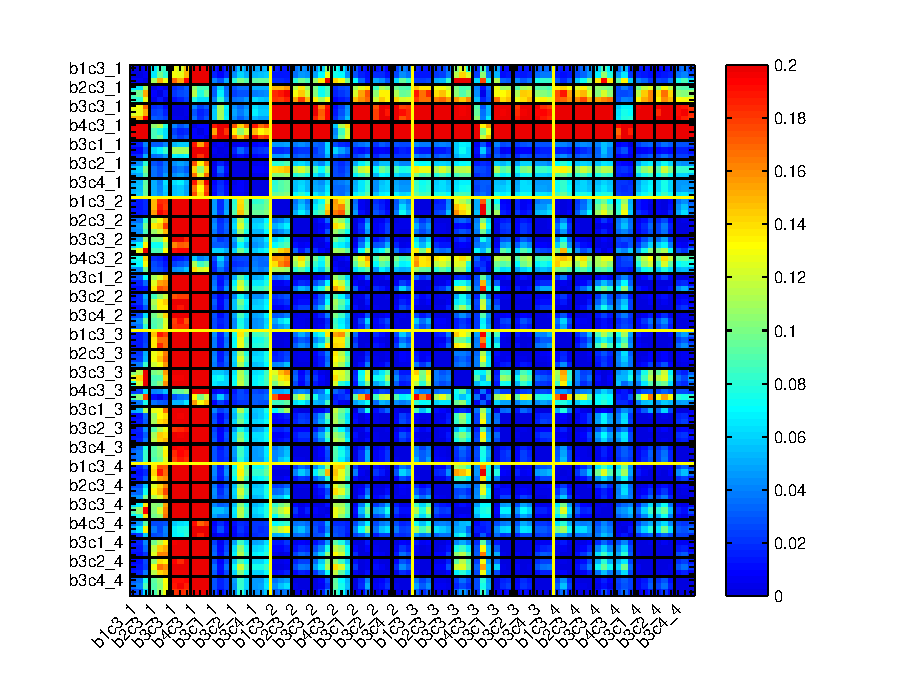
\includegraphics[width=18cm,height=18cm]{./fig/heatmap_all6_3.eps}
  \caption{ \scriptsize{A heatmap representation of the distance matrix of 84 time series (7 setups $\times$ 4 cycles $\times$ 3 trials). The labels are in the format of ``setup$\_$cycle''. For example, ``b1c3$\_$1'' represents the first cycle of the b1c3 setup. The yellow lines divide the x and y axis by the 4 cycles and hence form 16 big blocks. In each big block, the black lines divide the x and y axis by the 7 setups and hence form 49 small blocks. }
}
\label{fig:heatmap}
\end{figure*}

\begin{figure}
    \centering
    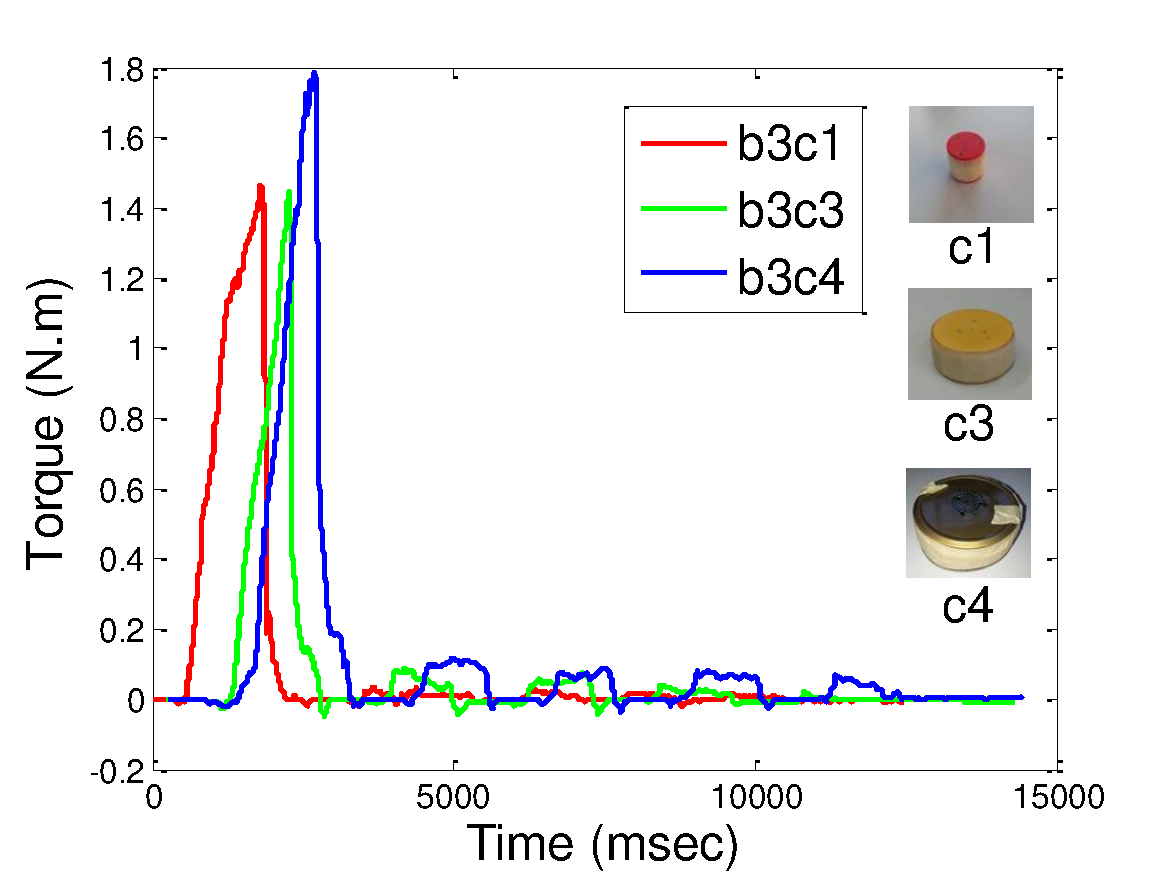
\includegraphics[width=8cm]{./fig/c1c3c4_time_T.pdf}
    \caption{ \scriptsize{Exert torque for opening bottle b3 with three different cap sizes.}
}
\label{fig:cappatterns}
\end{figure}


As mentioned before, the demonstration of each setup is repeated three times and the data from the same setup and same cycle are presumed to belong to the same cluster. To set a threshold for clustering, we check the distances between the time series come from the same setup and the same phase. The largest distance found is 0.04 (normalized) from the $b3c2$ phase 4. We add a $10\%$ margin on this (resulting to 0.044) and use it as the threshold of clustering. The time series distance less than the threshold are grouped into the same cluster. We use the hierarchical agglomerative clustering (Section~\ref{sec:cluster}) to merge the data into different clusters. After 5 times of merging, the clusters are not mergeable and 3 clusters remains.

These three clusters contain the data from:

\begin{enumerate}
\item phase I of $b4c3$ (most difficult bottle), 3 time series;
\item phase I of $b3c1, b3c2, b3c3, b3c4, b2c3$ and phase II of $b4c3$, 24 time series;
\item phase I of $b1c3$ (easiest bottle) and phase II of the other setups, 57 time series.
\end{enumerate}

The result of clustering is shown in Table~\ref{tab:cluster}. This result suggests that human use three different strategies for opening bottles: one for handling the phase I of the most difficult bottle with adhesive materials on the bottle and cap surfaces; one for handling the phase I of most bottles and the phase II of the most difficult bottle; and one for handling the phase I of the lubricated bottle and the phase II of the other bottles. The size of the cap turn out to be playing a less important role in the control strategies. According to this result, we encode these three clusters separately.


%\begin{table}
%\centering
%\renewcommand{\arraystretch}{1.5}
%    \begin{tabular}
%    %{|>{\centering\arraybackslash}p{2cm}|>{\centering\arraybackslash}p{1.2cm}|>{\centering\arraybackslash}p{1.7cm}|>{\centering\arraybackslash}p{1.2cm}|>{\centering\arraybackslash}p{1.5cm}|>{\centering\arraybackslash}p{1.5cm}|>{\centering\arraybackslash}p{1.7cm}|>{\centering\arraybackslash}p{1.7cm}|>{\centering\arraybackslash}p{0.9cm}|}
%    { | c |>{\centering\arraybackslash}p{10cm}|}
%    \hline
%    Cluster & Member time series \\ \hline
%    1       & $b4c2_1$  \\ \hline
%    2       & $b2c2_1,b3c2_1,b4c2_2,b4c2_3,b4c2_4,b2c3_1,b2c4_1$  \\ \hline
%    3       & $b1c2_1,b1c2_2,b1c2_3,b1c2_4,$
%             $  b2c2_2,b2c2_3,b2c2_4, $ \\
%    &         $  b3c2_2,b3c2_3,b3c2_4, $
%            $  b2c1_2,b2c1_3,b2c1_4, $ \\
%    &         $  b2c3_2,b2c3_3,b2c3_4, $
%             $  b2c4_2,b2c4_3,b2c4_4$  \\ \hline
%    \end{tabular}
%\caption{Clustering result}
%\label{tab:cluster}
%\end{table}


\begin{table*}
\centering
\begin{tabular}{p{1.4cm} p{1.4cm}|p{1.6cm} p{1.6cm} p{1.6cm}  p{1.6cm} }
& & \parbox[c]{1em}{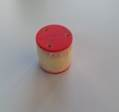
\includegraphics[width=1.5cm]{./fig/c1.jpg}}\newline Cap 1
& \parbox[c]{1em}{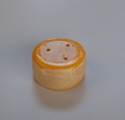
\includegraphics[width=1.5cm]{./fig/c2.jpg}}\newline Cap 2
& \parbox[c]{1em}{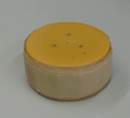
\includegraphics[width=1.5cm]{./fig/c3.jpg}}\newline Cap 3
& \parbox[c]{1em}{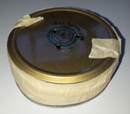
\includegraphics[width=1.5cm]{./fig/c4.jpg}}\newline Cap 4      \\ \hline
{\parbox[c]{1em}{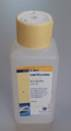
\includegraphics[width=1.5cm]{./fig/b1.jpg}}}
         & Phase I  &           &           & {\vspace{-0.7cm}}\pbox{2cm}{(b1c3) \\ Cluster 3} &           \\
Bottle 1 & Phase II &           &           &        Cluster 3 &           \\ \hline
{\parbox[c]{1em}{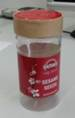
\includegraphics[width=1.5cm]{./fig/b2.jpg}}}
%         & Phase I  &{\vspace{-0.7cm}}\pbox{2cm}{(b2c1) \\Cluster 2} &{\vspace{-0.7cm}}\pbox{2cm}{(b2c2) \\Cluster 2} &{\vspace{-0.7cm}}\pbox{2cm}{(b2c3) \\Cluster 2} &{\vspace{-0.7cm}}\pbox{2cm}{(b2c4) \\Cluster 2} \\
%Bottle 2 & Phase II &       Cluster 3 &       Cluster 3 &       Cluster 3 &       Cluster 3 \\ \hline
         & Phase I  &           &           &{\vspace{-0.7cm}}\pbox{2cm}{(b2c3) \\Cluster 2} &           \\
Bottle 2 & Phase II &           &           &       Cluster 3 &           \\ \hline
{\parbox[c]{1em}{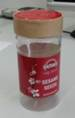
\includegraphics[width=1.5cm]{./fig/b3.jpg}} }
%         & Phase I  &           &           &{\vspace{-0.7cm}}\pbox{2cm}{(b3c3) \\Cluster 2} &           \\
%Bottle 3 & Phase II &           &           &       Cluster 3 &           \\ \hline
         & Phase I  &{\vspace{-0.7cm}}\pbox{2cm}{(b3c1) \\Cluster 2} &{\vspace{-0.7cm}}\pbox{2cm}{(b3c2) \\Cluster 2} &{\vspace{-0.7cm}}\pbox{2cm}{(b3c3) \\Cluster 2} &{\vspace{-0.7cm}}\pbox{2cm}{(b3c4) \\Cluster 2} \\
Bottle 3 & Phase II &       Cluster 3 &       Cluster 3 &       Cluster 3 &       Cluster 3 \\ \hline
{\parbox[c]{1em}{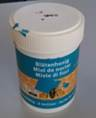
\includegraphics[width=1.5cm]{./fig/b4.jpg}}\newline }
         & Phase I  &           &           &{\vspace{-0.7cm}}\pbox{2cm}{(b4c3) \\Cluster 1} &           \\
Bootle 4 & Phase II &           &           &       Cluster 2 &           \\ \hline
\end{tabular}
\caption{Clustering result}
\label{tab:cluster}
\end{table*}

%\begin{figure}
%\label{forcecluster}
%  \centering
%  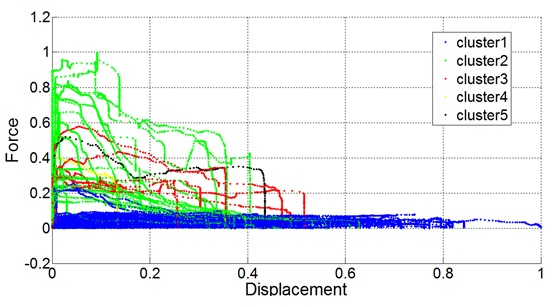
\includegraphics[width=11cm]{./fig/forcecluster.jpg}
%  \caption{ \scriptsize{Hierarchal clustering result.}
%}
%\end{figure}

\subsubsection{Learning Modules}
\label{sec:module}
We encode the data in each of the module by GMM. As explained in Section~\ref{sec:model}, a forward model and an inverse model are built for each module. The forward model is encoded by the joint distribution $p\{s_t,s_{t-1},a_{t-1}\mid\Omega_F\}$, while the inverse model is encoded by $p\{s_t,s{t+1},a_t,a_{t-1}\mid\Omega_I\}$. For each model, the number of Gaussians is determined by the Bayesian information criterion (BIC). We use 25 Gaussian for cluster 1, 40 for cluster 2 and 15 for cluster 3. Their BIC tests are shown in Fig~\ref{fig:bic}.

\begin{figure}
  \centering
  \subfloat[\scriptsize{Cluster 1. Optimal number of Gaussians is 25.}]{\includegraphics[width=6cm]{./fig/bic_cluster1_2.eps}}

  \subfloat[\scriptsize{Cluster 2. Optimal number of Gaussians is 40.}]{\includegraphics[width=6cm]{./fig/bic_cluster2_2.eps}}

  \subfloat[\scriptsize{Cluster 3. Optimal number of Gaussians is 15.}]{\includegraphics[width=6cm]{./fig/bic_cluster3_2.eps}}

  \caption{ \scriptsize{BIC test result for clusters. }
}

\label{fig:bic}
\end{figure}

%\begin{table}
%\centering
%\renewcommand{\arraystretch}{1.5}
%    \begin{tabular}
%    %{|>{\centering\arraybackslash}p{2cm}|>{\centering\arraybackslash}p{1.2cm}|>{\centering\arraybackslash}p{1.7cm}|>{\centering\arraybackslash}p{1.2cm}|>{\centering\arraybackslash}p{1.5cm}|>{\centering\arraybackslash}p{1.5cm}|>{\centering\arraybackslash}p{1.7cm}|>{\centering\arraybackslash}p{1.7cm}|>{\centering\arraybackslash}p{0.9cm}|}
%    { | c | c | c | c | c |}
%    \hline
%    Cluster & Forward Model &  Inverse Model \\ \hline
%    1       & 98.1\%  & 13.8     \\ \hline
%    2             & 92.1\%  & 21.9    \\ \hline
%    3              & 91.0\%  & 16.0    \\ \hline
%    \end{tabular}
%\caption{Number of Gaussians in each GMM}
%\label{tab:GMM}
%\end{table}


\subsection{Generating motor command for manipulation}
\label{sec:command}
Our approach is independent of robot system and can potentially be applied to any robot. We choose to implement this work with a Barrett hand mounted on a KUKA lightweight robot as they are available in our lab. We implement the multiple module system on this platform to enable the robot opening bottle caps.

\begin{algorithm}
  \caption{Control Algorithm}
  \begin{algorithmic}[1]
    \For{r = 1:4}
    \State REACHING(): Robot move to initial position\;
        \Function{TURNING()}{} %      \Comment{$\oplus$: bit}
          \State Read previous sensor information $\{s_{t-1},\tau_{t-1},F_{t-1}\}$\;
          \For{k=1:3}
            \State $\hat{s}^{k}$ = FORWARD($s_{t-1},T_{t-1},\Omega_I^k$) \;
          \EndFor
          \For{k=1:3}
            \State $\lambda{k}$ = ResponsibilityFactor($\hat{s}^{k},s_t$) \;
          \EndFor
          \State Read current sensor information $\{s_{t}\}$\;
          \For{k=1:3}
            \State $\{a^k\}$ = INVERSE($s*_{t+1},s_t,a_{t-1}$) \;
          \EndFor
          \State $\{a_t\} = \sum_{k=1,2,3}\lambda{k}\{a^k\}$\;\;
          \State Add compensational torque to $\tau_t$\;
          \State Execute motor command $\{a_t\}$ \;
          \State RELEASING(): Release the cap;
        \EndFunction
    \EndFor

    \While{LIFTCAP() is false}
        \State REACHING();
        \State TURNING();
        \State RELEASING();
    \EndWhile

  \end{algorithmic}
  \label{code:control}
\end{algorithm}


In this experiment, we control the wrist joint (last joint of KUKA) for producing torque to turn the bottle cap. A force torque sensor is fixed under the bottle to provide torque feedback. Each finger of the Barrett hand is mounted with a $Syntouch$\footnote{http://www.syntouchllc.com/} tactile sensor, which is calibrated to provide contact force information, for the grip force feedback. The cap displacement is measured by the wrist joint displacement, assuming that there is no slip between the fingers and the cap.

The target bottle is fixed on the top of a table with it's cap tighten. The robot is placed above it on a distance that allows a proper grasp on the cap. The Barrett hand then close the fingers until the bottle cap is touched. This position is recorded as the initial position, where the cap displacement is marked as zero. In the experiment we focus on the turning cycle. The releasing and reaching cycles are programmed by opening the fingers and restoring to the initial position.

We first test the model with the trained bottles and then test with two new bottles. With each bottle, the turning-releasing-restoring cycles are repeated four times. Data stream from the sensors are filtered to $100Hz$. Once the turning cycle starts, the forward models take the torque and displacement at the last time step as input, compute the expected displacement of the current time step. These expected displacements are compared with the actual displacement measured at the sensor to evaluate the reliability, expressed as a normalized responsibility factor, of each module. The inverse models take the current displacement, desired next displacement and the previous force and torque as input to compute the a proper action (force and torque) to take on the cap. Each of the three outputs is multiplied with its responsibility factor, and the final output is the sum of the factorized three outputs (Algorithm~\ref{code:control}).

In implementation on a real robot, we found that without putting any restriction of the responsibility factor, it can change rapidly. This is caused by the environmental noise in the sensory input and results in instability of the control system. We apply a low pass filter on the responsibility factor to reduce the fluctuation. This filtering implies that the real dynamics does not switch with high frequency, which consists with the character of our task. %(Figure.~\ref{fig:rf}).

%\begin{figure}
%  \centering
%  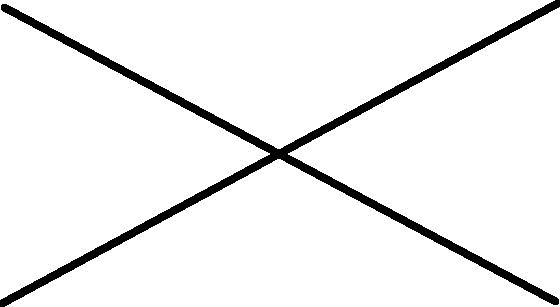
\includegraphics[width=2cm]{./fig/void.jpg}
%  \caption{ \scriptsize{Filtered responsibility factor. (TODO)}
%}
%\label{fig:rf}
%\end{figure}

Before apply the final output on the robot, a compensational torque is added to it in order to compensate the slag causing by the distortion of the robot hand during turning. The control algorithm described above is shown in algorithm~\ref{code:control}.



\subsection{Experiment results}


% TODO:
% 1) explain whether the use of the clusters correspond to your expectations and really relate to an identification of different phases
% 2) what the novel object consist of, in what do they differ from the other objects
% 3) what were your expectations in terms of cluster use for these new objects
% 4) Do the results match your expectations

%We implement this algorithm with two bottles (b1 and b4) in the training set and then two bottles (b5 and b6) had not been used for training.
We validated the algorithm to control cap opening in our robot. We first tested the ability of the system to open 2 of the bottles seen during training (b1 and b4). We then tested the generalization capacity of the system by opening two bottles (b5 and b6) not seen during training.
Bottle b1 and b4 are the easiest and most difficult bottle to open in the training set.
Bottle b5 is a large bottle, which is hard for human to grab and open. Bottle b6 is a glass bottle with a plastic cap. The surface interaction between these two materials is not demonstrated. As the Barrett hand is significantly larger than a human hand, $b1, b4, b6$ are mounted with $c5$ (the cap of $b5$ with diameter $110 mm$) on the top to ensure a firm grasp. In total 4 different setups are used in the experiment: $b1c5, b4c5, b5c5$ and $b6c5$. As discuss above, the size of the cap has minor effect on the control strategy. Therefore we expect the setups $b1c5$ and $b4c5$ will result in a similar behavior as those of $b1c3$ and $b4c3$ in the training. The experimental results and demonstration snapshots are shown in figures~\ref{fig:demo_b1}-~\ref{fig:demo_b6}~\footnote{Demonstration videos are available at http://www.cs.bath.ac.uk/~bh325/opencap.rar}. Figure~\ref{fig:demo_b1b4b5b6} is a similar plot to figure~\ref{fig:bottlepatterns}, that aligns the exert torque of the 4 experiments.

In each experiment we record the cap displacement, exert torque, and the responsibility factors of all three modules. Bottle b1 is the easiest bottle to open in the training set, the control policies of both phase $I$ and phase $II$ are grouped into cluster 3. As a result, in the b1 experiment the cluster 3 takes most responsibility (Figure.~\ref{fig:demo_b1}).

Bottle b4 is the most difficult bottle to open in the training set and it's phase $I$ requires more than 3 $Nm$ (Figure.~\ref{fig:bottlepatterns}). Due to the smooth contact surfaces between the Barrett hand and the cap, it is difficult to apply 3 $Nm$ torque to the cap without slipping. To avoid damaging the robot, we test the b4 phase $II$ only: the cap is loosely screwed on the bottle. Without knowing this, in the experiment the robot is able to properly estimate the current task context. As can be seen from the figure~\ref{fig:demo_b4}, different from b1, the dominate cluster is the cluster 2 which corresponds to the b4 phase II. This performance would be hard to achieved by a deterministic system based on expected values for friction coefficients.

Bottle b5 is a novel one but is made of similar material (plastic) to the trained bottles. A very similar torque profile to b2 and b3 is generated for b5: phase $I$ is sharp, while phase $II$ is flatten and significantly smaller than phase $I$ (b2: Figure.~\ref{fig:bottlepatterns}, b3: Figure.~\ref{fig:cappatterns}, b5: Figure.~\ref{fig:demo_b5}). This is because b5 has dry contact surface as b2 and b3, and b1 is lubricated and b4 is attached with sticky material, i.e. honey.

Bottle b6 is also a novel one but with novel surface materials (plastic and glass)~\footnote{A common way of measuring the FCO of a material is measuring it against metal: the static FCO between glass and metal is 0.5-0.7, while between two polythene and steel is around 0.2. This implies that the plastic and glass are indeed very different in FCO. There is not an universal measurement of the FOC between plastic and glass.}. It's torque profile is different from what we observed in training set. Despite this, b6 is open with this torque profile generated by the three learnt modules.

% TODO: In all actions, cluster 2 is always firstly selected as the dominate module.

With the above four different setups, the modular model adapts accordingly and successfully generate torque command to open the bottles. Successful cap opening is achieve when the cap is unscrewed far enough that it can be lifted up. Though no prior information is provided about the bottles, the task contexts are properly estimated and ``contextized'' motor commands are generated to unscrew the caps. These experiments show that our multiple modular approach is indeed effective in manipulation tasks.



\begin{figure*}
  \centering
  \vspace{0.8cm}
  \subfloat[\scriptsize{Snapshots for robot opening b1 demonstration.}]
  {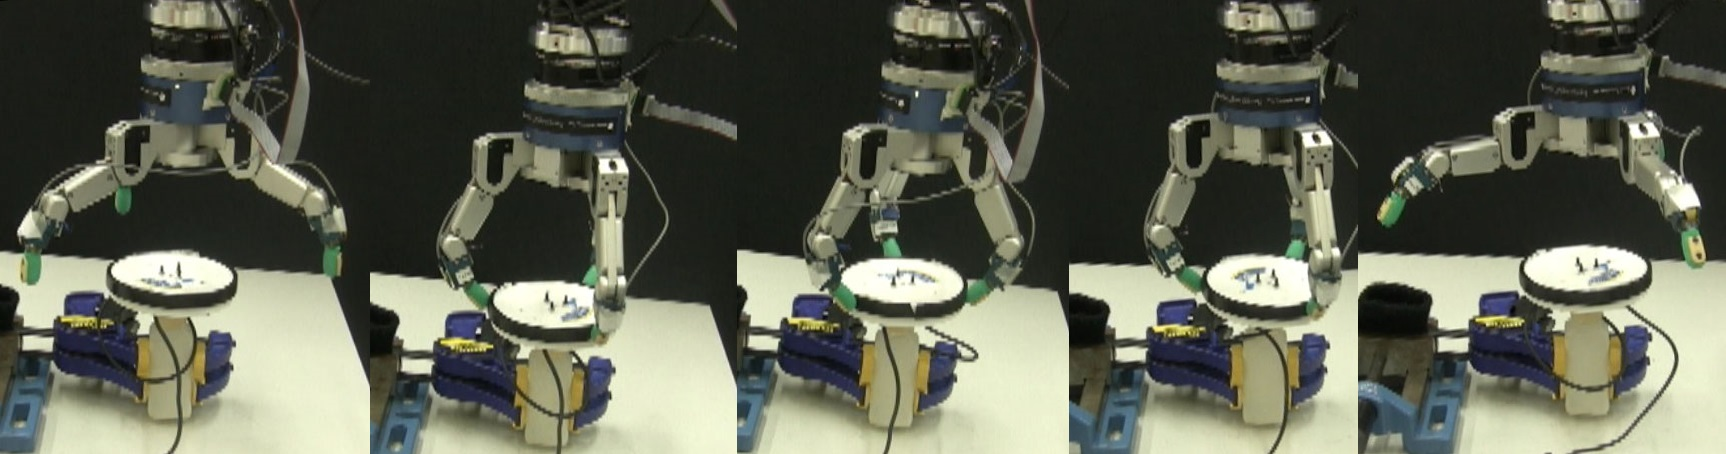
\includegraphics[width=15cm]{./fig/demo_b1.jpg}}

  \vspace{0.3cm}
  %\hspace{0.2cm}
  \subfloat[\scriptsize{Cap displacement during the demonstration. }]
  {
\includegraphics[width=15cm]{./fig/demo_b1_s.eps}}

  \vspace{0.3cm}
  \hspace{-0.3cm}
  \subfloat[\scriptsize{Exert torque against cap displacement during the demonstration.}]
  {
\includegraphics[width=15cm]{./fig/demo_b1_T.eps}}

  \vspace{0.3cm}
  %\vspace{0.5cm}
  \subfloat[\scriptsize{Responsibility factor against cap displacement of each module.}]
  {
\includegraphics[width=15cm]{./fig/demo_b1_rf.eps}}
  \caption{ \scriptsize{Robot demonstration on opening b1.}
}

\label{fig:demo_b1}
\end{figure*}

\begin{figure*}
  \centering
  \vspace{0.8cm}
  \subfloat[\scriptsize{Snapshots for robot opening b4 demonstration.}]
  {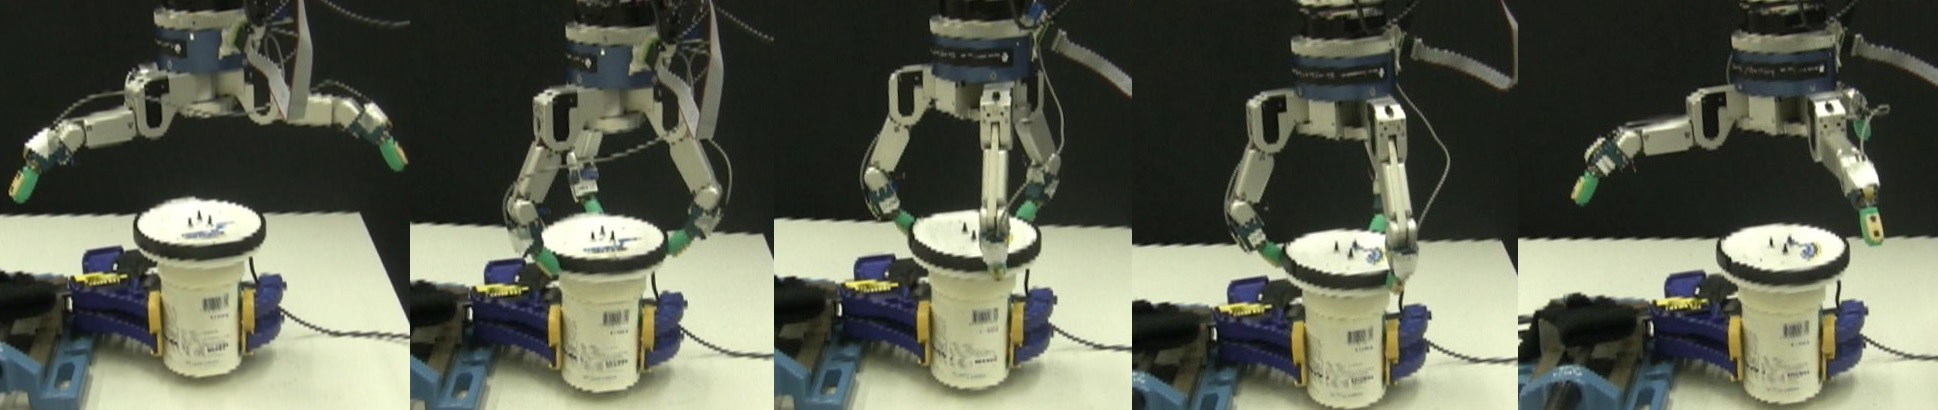
\includegraphics[width=15cm]{./fig/demo_b4.jpg}}

  \vspace{0.3cm}
  %\vspace{0.5cm}
  \subfloat[\scriptsize{Cap displacement during the demonstration. }]
  {
\includegraphics[width=15cm]{./fig/demo_b4_s.eps}}

  \vspace{0.3cm}
  \hspace{-0.2cm}
  \subfloat[\scriptsize{Exert torque against cap displacement during the demonstration.}]
  {
\includegraphics[width=15cm]{./fig/demo_b4_T.eps}}

  \vspace{0.3cm}
  %\vspace{0.5cm}
  \subfloat[\scriptsize{Responsibility factor against cap displacement of each module.}]
  {
\includegraphics[width=15cm]{./fig/demo_b4_rf.eps}}

  \caption{ \scriptsize{Robot demonstration on opening b4.}
}
\label{fig:demo_b4}
\end{figure*}

\begin{figure*}
  \centering
  \vspace{0.8cm}
  \subfloat[\scriptsize{Snapshots for robot opening b5 demonstration.}]
  {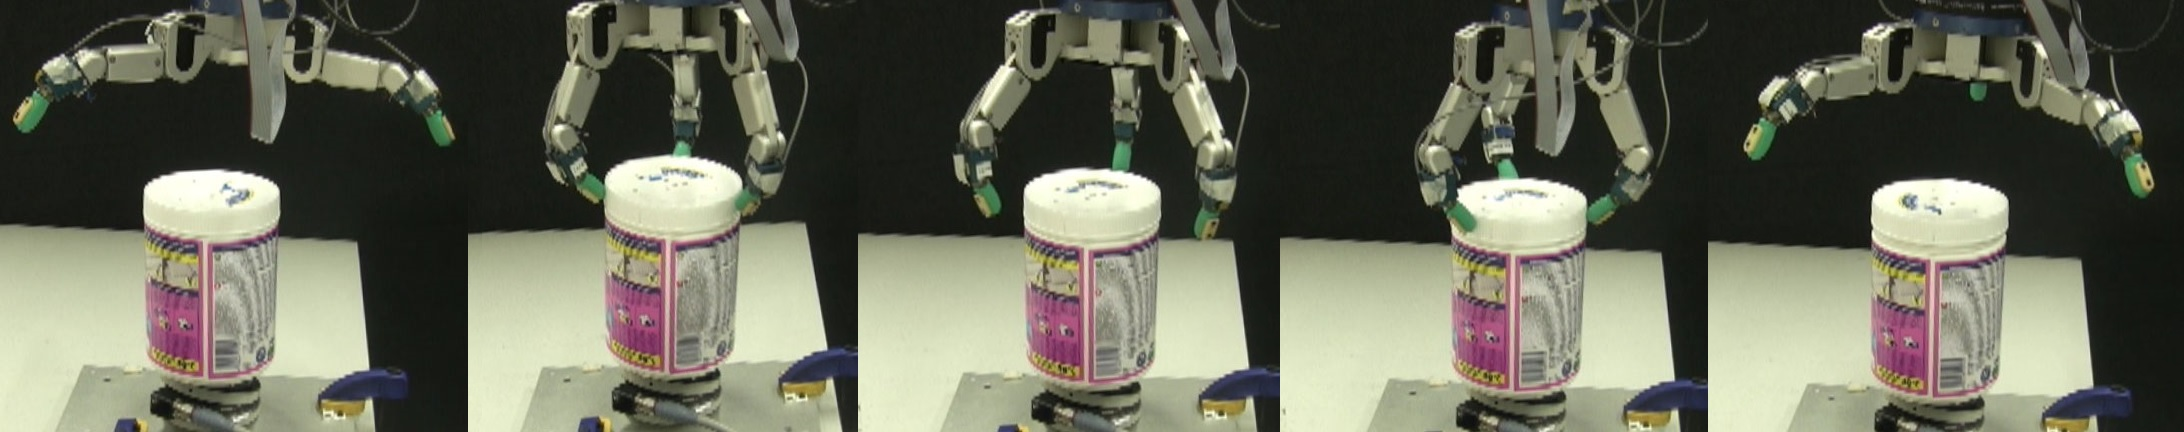
\includegraphics[width=15cm]{./fig/demo_b5.jpg}}

  \vspace{0.3cm}
  %\vspace{0.5cm}
  \subfloat[\scriptsize{Cap displacement during the demonstration.}]
  {
\includegraphics[width=15cm]{./fig/demo_b5_s.eps}}

  \vspace{0.3cm}
  %\vspace{0.5cm}
  \subfloat[\scriptsize{Exert torque against cap displacement during the demonstration.}]
  {
\includegraphics[width=15cm]{./fig/demo_b5_T.eps}}

  \vspace{0.3cm}
  %\vspace{0.5cm}
  \subfloat[\scriptsize{Responsibility factor against cap displacement of each module.}]
  {\includegraphics[width=15cm]{./fig/demo_b5_rf.eps}}

  \caption{ \scriptsize{Robot demonstration on opening a new bottle (b5).}
}
\vspace{5cm}
\label{fig:demo_b5}
\end{figure*}

\begin{figure*}
  \centering
  \vspace{0.8cm}
  \subfloat[\scriptsize{Snapshots for robot opening b6 demonstration.}]
  {\includegraphics[width=15cm]{./fig/demo_b6.jpg}}

  \vspace{0.3cm}
  %\vspace{0.5cm}
  \subfloat[\scriptsize{Cap displacement during the demonstration.}]
  {\includegraphics[width=15cm]{./fig/demo_b6_s.eps}}

  \vspace{0.3cm}
  \hspace{-0.5cm}
  \subfloat[\scriptsize{Exert torque against cap displacement during the demonstration.}]
  {\includegraphics[width=15cm]{./fig/demo_b6_T.eps}}

  \vspace{0.3cm}
  %\vspace{0.5cm}
  \subfloat[\scriptsize{Responsibility factor against cap displacement of each module.}]
  {\includegraphics[width=15cm]{./fig/demo_b6_rf.eps}}

  \caption{ \scriptsize{Robot demonstration on opening a new bottle (b6).}
}
\label{fig:demo_b6}
\end{figure*}


\begin{figure}
  \centering
  \includegraphics[width=8cm]{./fig/rb1b4b5b6_time_T.eps}
  \caption{ \scriptsize{Robot exert torque for opening four bottles: b1 b4 b5 b6. Time is warped and shifted for displace purpose.}
}
\label{fig:demo_b1b4b5b6}
\end{figure}


%A set of snapshots of the implementations are shown in Figure.~\ref{fig:demo_train} and~\ref{fig:demo_new}. Figure.~\ref{fig:demo_result} shows the sensory data from these demonstrations.

%\begin{itemize}
%  \item Demonstration on the learnt bottles \ldots
%  \item Demonstration on a new bottle \ldots
%  \item Filtering noise  \ldots
%  \item different module's rf
%\end{itemize}

%\begin{figure}
%  \centering
%  \includegraphics[width=15cm]{./fig/demo_train.jpg}
%  \caption{ \scriptsize{Robot demonstration on opening a trained bottle cap. (TODO)}
%}
%\label{fig:demo_train}
%\end{figure}
%
%\begin{figure}
%  \centering
%  \includegraphics[width=15cm]{./fig/demo_new.jpg}
%  \caption{ \scriptsize{Robot demonstration on opening a new bottle cap. (TODO)}
%}
%\label{fig:demo_new}
%\end{figure}
%
%\begin{figure}
%  \centering
%  \includegraphics[width=2cm]{./fig/void.jpg}
%  \caption{ \scriptsize{Robot demonstration data. (TODO)}
%}
%\label{fig:demo_result}
%\end{figure} 